% !TEX program = pdflatex
% 4.11   2.14  2.11 3.13  lemma 6.8    lemma 6.9 
\documentclass{article}
\DeclareMathAlphabet{\mathpzc}{OT1}{pzc}{m}{it}
\setlength{\parindent}{0pt}
\usepackage[table]{xcolor}
\usepackage{graphicx}
\usepackage{amssymb}
\usepackage{amsmath}
\usepackage{amsthm}
\usepackage{hyperref}
\usepackage{pgfplots}
\usepackage{pst-plot}
% \usepackage{fdsymbol}
\usepackage{empheq}
\usepackage{tikz}
\usepackage[most]{tcolorbox}
\usepackage{enumerate}
\usepackage{scalerel}
\usepackage{relsize}
\usepackage{mdframed}
\usepackage[utf8]{inputenc}
% \usepackage[margin=1.3in]{geometry}
\usetikzlibrary{positioning}


\usetikzlibrary{calc,patterns,angles,quotes}
\definecolor{myblue}{rgb}{2.55, 1.50, 0.20}
% \definecolor{myblue}{RGB}{227, 234, 253}
\newtcbtheorem[number within=subsection]{mytheo}{Sats}%
    {colback=myblue!15,colframe=black!30!black,
     enhanced,
     coltitle=black!75!black, boxrule=0.8pt,
     attach boxed title to top left=
       {xshift=2ex,yshift=-2mm,yshifttext=-1mm},
     boxed title style={colframe=black!30!black, boxrule=0.8pt,
       colback=myblue!60}}{th}

\newtcbtheorem[number within=subsection]{mydef}{Definition}%
    {colback=myblue!15,colframe=black!30!black,
     enhanced,
     coltitle=black!75!black, boxrule=0.8pt,
     attach boxed title to top left=
       {xshift=2ex,yshift=-2mm,yshifttext=-1mm},
     boxed title style={colframe=black!30!black, boxrule=0.8pt,
colback=myblue!60}}{th}

\newtcbtheorem[number within=subsection]{myprop}{Proposition}%
    {colback=myblue!15,colframe=black!30!black,
     enhanced,
     coltitle=black!75!black, boxrule=0.8pt,
     attach boxed title to top left=
       {xshift=2ex,yshift=-2mm,yshifttext=-1mm},
     boxed title style={colframe=black!30!black, boxrule=0.8pt,
colback=myblue!60}}{th}

\newtcbtheorem[number within=subsection]{mykol}{Korollarium}%
    {colback=myblue!15,colframe=black!30!black,
     enhanced,
     coltitle=black!75!black, boxrule=0.8pt,
     attach boxed title to top left=
       {xshift=2ex,yshift=-2mm,yshifttext=-1mm},
     boxed title style={colframe=black!30!black, boxrule=0.8pt,
colback=myblue!60}}{th}

\newtcbtheorem[number within=subsection]{mylemma}{Lemma}%
    {colback=myblue!15,colframe=black!30!black,
     enhanced,
     coltitle=black!75!black, boxrule=0.8pt,
     attach boxed title to top left=
       {xshift=2ex,yshift=-2mm,yshifttext=-1mm},
     boxed title style={colframe=black!30!black, boxrule=0.8pt,
colback=myblue!60}}{th}

% ---------------------------------------------
% ---------------RE-NEW COMMAND----------------
% ---------------------------------------------
\newcommand\mul[1]{\multicolumn{1}{c}{#1}}
\setlength{\parskip}{1em}
\renewcommand{\baselinestretch}{1.2}
\renewcommand*{\proofname}{Bevis}
\newcommand{\ovning}[1]{\noindent {\bf Övning #1.}}
\renewcommand{\contentsname}{Innehåll}
\newcommand{\orbit}[0]{\mathlarger{\mathlarger{\mathcal{O}}}}
\newcommand{\grad}[0]{\textnormal{deg}}
\newcommand{\im}[0]{\textnormal{im}}
\newtheorem{definition}{Definition}[section]
\pgfplotsset{compat=1.8}

\theoremstyle{definition}
\newtheorem{thm}{Theorem}[section]
\newtheorem{exmp}[thm]{Exempel}
\begin{document}


% \begin{figure}

%   % center everything in the figure
%   \centering
%   % horizontal node distance
%   \newcommand{\mydistance}{.6cm}
%   \begin{tikzpicture}[node distance=2cm, scale=1]
%     \draw[fill=myblue!60] (-6,2) rectangle (6,-8);
%   % \title{Untergruppenverband der $A_4$}
%   \node(A4)                           {$A_4$};
%   \node(V4)       [below right=2cm and 2cm of A4] {$V_4$};
%   \node(C31)      [below left=2cm and 0cm of A4]  {$C_3$};
%   \node(C32)      [left=\mydistance of C31]       {$C_3$};
%   \node(C33)      [left=\mydistance of C32]       {$C_3$};
%   \node(C34)      [left=\mydistance of C33]       {$C_3$};
%   \node(C22)      [below=2cm of V4]       {$C_2$};
%   \node(C21)      [left=\mydistance of C22]       {$C_2$};
%   \node(C23)      [right=\mydistance of C22]      {$C_2$};
%   \node(1)            [below=6cm of A4]     {$\left\{1\right\}$};
%   \draw(A4)       -- (V4);
%   \foreach \x\y in {1,2,3,4} {
%       \draw (A4) -- (C3\x);
%       \draw (C3\x) -- (1);
  
%   }
%   \foreach \x\y in {1/2,2/3,3/4} {
%       \draw(V4) -- (C2\x);
%   \draw (C3\x) -- (C3\y);
%   \draw (C2\x) -- (1);
%   }
%   \draw(C21)      -- (C22);
%   \draw(C22)      -- (C23);
%   \end{tikzpicture}
%   % \caption{Untergruppenverband}
%   \end{figure}

\begin{figure}
  \begin{center}
    \newcommand{\mydistance}{.6cm}
    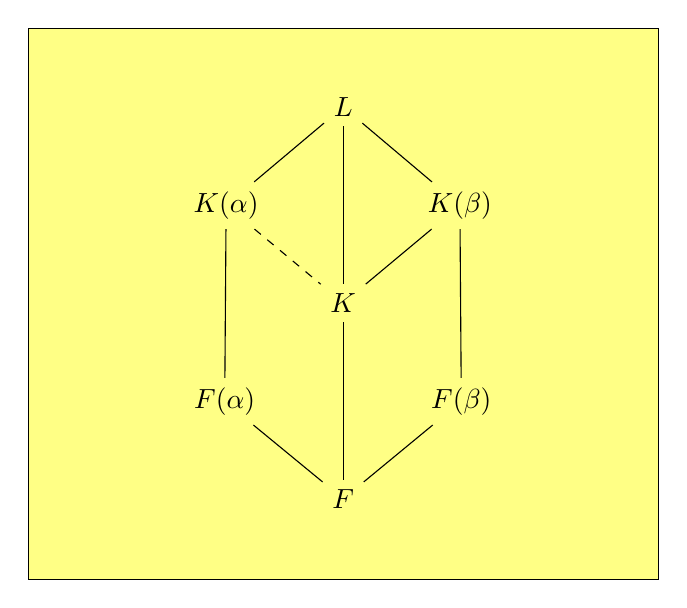
\begin{tikzpicture}[node distance=2cm, scale=1]
    \draw[fill=myblue!60] (-4,1) rectangle (4,-6);
    \node(L) {$L$};
    \node(Ka) [below left=1cm of L] {$K(\alpha)$};
    \node(Kb) [below right=1cm of L] {$K(\beta)$};
    \node(K) [below=2cm of L] {$K$};
    \node(F) [below=2cm of K] {$F$};
    \node(Fa) [below left=1 of K] {$F(\alpha)$};
    \node(Fb)[below right = 1 of K] {$F(\beta)$};  
  
    \draw[dashed](Ka) -- (K);
    \draw(Kb) -- (K);
    \draw(L) -- (Ka);
    \draw(L) -- (Kb);
    \draw(K) -- (L);
    \draw(F) -- (K);
    \draw(Ka) -- (Fa);
    \draw(Fa) -- (F);
    \draw(Fb) -- (F);
    \draw(Kb) -- (Fb);
    \end{tikzpicture}
  \end{center}  
\end{figure}
\title{%
  Galoisteori och de olösbara polynomen \\
  \small{En introduktion till det abstrakta - Del II}
}
\author{Gabriel Rajkowski}
\date{\today}
\maketitle
\begin{center}
  \begin{tabular}{l r}
  Skola: & Europaskolan \\ 
  Program: & Scienceprogramet \\ 
  Handledare: & Johan Wild
  \end{tabular}
\end{center}
(Denna figur är temporär. Jag ska byta ut den mot ett annat diagram när jag kommer in på Galoisteorin)

\thispagestyle{empty}
  
\clearpage
\tableofcontents
\section{Inledning}
Här ska jag snabbt nämna att detta är del 2 och är en forstättning till del 1 (Banach-Tarski paradoxen). 
(Fler övningar och exempel ska komma. Detta fixar jag efter allt annat är klart.)
\section{Historia}
Berätta lite om Galoisteorins historia. 
\section{Komplement till del I}
Denna del ägnar sig åt saker som inte togs upp i del I på grund av de inte fick plats eller som inte var nödvändiga men som kommer att komma 
till hands i denna del.

\subsection{Linjär algebra}
En stor sak som undveks i del I var vektorrum. Det visar sig faktiskt att vektorrum blir väldigt praktiska och går hand i hand med andra 
algebraiska strukturer såsom kroppar och dess utvidgningar. I detta delavsnitt kommer vi att studera grunderna för vektorrum så att de senare kan användas till 
våran fördel.

\begin{mydef}{Vektorrum}{}
  Ett vektorrum över en kropp (vi definerar detta senare) $F$ är en mängd $V$ under addition och subtraktion som uppfyller följande axiom.
  \begin{enumerate}[I)]
    \item $V$ skapar en abelsk grupp under addition,
    \item $a \cdot (b \cdot v) = (a \cdot b) \cdot v$,
    \item $1 \cdot v = v$ där 1 är den multiplikativa enhetselementet i $F$,
    \item $a \cdot (u + v) = (a \cdot u) + (a \cdot v)$,
    \item $(a + b) \cdot v = (a \cdot v) + (b \cdot v$),
  \end{enumerate}
  där $a, b \in F$ och $v, u \in V$.
\end{mydef}
Elementen i $F$ brukar kallas för skalärer och elementen i $v$ 
brukar kallas för vektorer. 

% \begin{mydef}{Linjära beroenden}{}
%   Låt $v_1, v_2, \cdots, v_n$ vara element i ett vektorrum 
%   $V$ över en kropp $F$ och låt $a_1, a_2, \cdots, a_n \in F$.
%   Vektorerna är \textit{linjärt oberoende} om ekvationen 
%   \[a_1v_1 + a_2v_2 + \cdot + a_nv_n = 0\]
%   endast har lösningen $a_1 = a_2 = \ldots a_n = 0$.
%   Om sådant inte är fallet, det vill säga då 
%   en vektor kan skrivas som en linjär kombination av de andra, 
%   så är vektorerna \textit{linjärt beroende}.
% \end{mydef}
(några exempel)

\begin{mydef}{Baser}{}
  En delmängd $K$ av ett vektorrum $V$ över en kropp $F$ är en \textit{bas} för $V$ om följande villkor uppfylls.  
  \begin{enumerate}[I)]
    \item $K$ är \textit{linjärt oberoende}. För $v_1, \ldots, v_n \in K$ och $a_1, \ldots, a_n \in F$ så har ekvationen 
    \[a_1v_1 + \cdots + a_n v_n = 0\]
    lösningen $a_1 = \cdots = a_n = 0$.
    \item $K$ \textit{spänner upp} $V$. För alla $v \in V$ så existerar det $b_1, \ldots b_m \in F$ och $v_1, \ldots v_m \in K$ så att 
    $v = b_1 v_1 + \cdots + b_m v_m$.
  \end{enumerate}
\end{mydef}

\subsection{Gruppteori}
Detta avsnitt kommer ägna sig åt normala delgrupper och kvotgrupper. Dessa blir mycket nödvändiga för oss när vi ska bevisa textens viktigaste sats. 
Mer specifikt kommer vi vara intresserade av kedjor av normala delgrupper och om deras kvotgrupp är abelsk eller icke. Denna 
del kommer även underlätta senare koncept inom ringteori.

\begin{mydef}{Normala delgrupper}{}
  Låt $N$ vara en delgrupp till $G$. Vi säger att $N$ är 
  en \textit{normal delgrupp} till $G$ om $N$ är 
  \textit{invariant under kojugering}, för alla $n \in N$ och 
  alla $g \in G$ så är $gng^{-1} \in N$. Vi skriver då $N \triangleleft G.$
\end{mydef}
Motivationen bakom denna till synes konstiga definition finner man i kvotgrupper. 
En definerande egenskap hos normala delgrupper tas upp i följande proposition.

\hypertarget{prop1}{}
\begin{myprop}{}{}
  Låt $N$ vara en normal delgrupp till $G$ och $g \in G$. Vänstersidoklassen till $N$ är då lika med högersidoklassen till $N$ med avseende på $g$, 
  $gN = Ng.$
\end{myprop}
(Väldigt kladdigt bevis. Fixar detta senare.)
\begin{proof}
  Om $n \in N$ så är $gn \in gN$. Notera nu att 
  \begin{equation*}
    gn = gn(g^{-1}g) = \underbrace{(gng^{-1})}_{ \substack{N \triangleleft G  \implies \\ gng^{-1} \in N}} g.
  \end{equation*}
  Detta visar att $gN \subseteq Ng.$ Ett godtyckligt element i $Ng$ är på formen $ng$. Observera att 
  \begin{equation*}
    ng = n(g^{-1})^{-1} = g \underbrace{g^{-1} {n(g^{-1})^{-1}}}_{\substack{N \triangleleft G  \implies \\ g^{-1} {n(g^{-1})^{-1} \in N}}}.
  \end{equation*}
  Detta visar att $Ng \subseteq gN$ vilket slutför beviset.
\end{proof}

\begin{mydef}{Kvotgrupper}{}
  Låt $N$ vara en normal delgrupp till $G$. \textit{Kvotgruppen} $G/N$, som utläses "$G$ modulo (mod) $N$", är gruppen innehållande alla 
  sidoklasser till $N$, 
  \[G/N \equiv \{gN \; | \; g \in G\},\]
  där gruppoperationen defineras som $(aN) (bN) = (ab)N$. 
\end{mydef}
Denna definition använder sig av vänstersidoklasser men, enligt \hyperlink{prop1}{proposition 3.2.1}, så kan man lika gärna använda sig 
av högersidoklasser. Notera att för $a' \in aN, a \in G$ så är $a'N = aN$ enligt resultat från del I. Det vi har kvar att visa är att $(a'N) (b'N) = (ab)N
\iff (a'b')N = (ab)N$, det vill säga att det inte spelar någon roll vilka representanter framför $N$, $a' \in aN, b' \in bN$, vi väljer. Resultatet av 
operationen bör vara oberoende av vilka representanter vi väljer, annars skulle det kunna finnas flera svar till en och samma sak. Med 
andra ord måste vi visa att operationen är \textit{väldefinerad}.

För att visa detta kan vi låta $a' \in aN$ och $b' \in bN$. Vi kan skriva dessa som $a' = an_1$ och $b' = bn_2$ för $n_1, n_2 \in N$. Med denna 
omskrivning kan vi konstatera att
\[(a'b')N = (an_1bn_2)N.\]
Eftersom assosiativitet gäller så är 
\[(an_1bn_2)N = an_1b(n_2N).\]
Vidare har vi även att $n_2 \in N$ vilket enligt resultat från del I ger 
\[an_1b(n_2N) = an_1bN.\]
Enligt \hyperlink{prop1}{proposition 3.2.1} har vi att 
\[an_1bN = ab(n_1N) = (ab)N.\]

Vi vet från del I att mängden av sidklasser utgör en partition av en grupp och därför är följande figur lämplig.

\begin{center}
  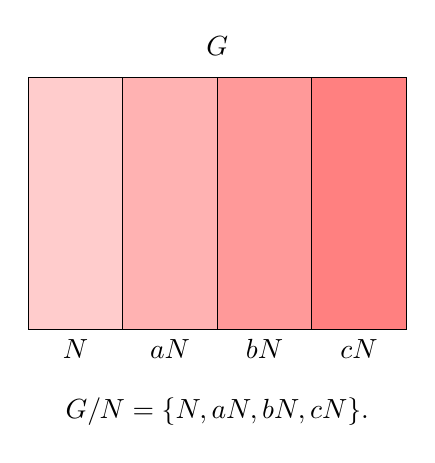
\begin{tikzpicture}[scale=0.8]
    \node at (0, 2.5) {$G$};
    \draw (-3,2) rectangle (3,-2);
    \foreach \i [count=\xi] in {-3, -1.5,..., 0}{
      \draw (\i, 2) rectangle (-\i, -2);
    }
    \node at (-2.25, -2.3) {$N$};
    \node at (-0.75, -2.3) {$aN$};
    \node at (0.75, -2.3) {$bN$};
    \node at (2.25, -2.3) {$cN$};
    \node at (0, -3.3) {$G/N = \{N, aN, bN, cN\}.$};

    \draw[fill = red!20] (-3, 2) rectangle (-1.5, -2);
    \draw[fill = red!30] (-1.5, 2) rectangle (0, -2);
    \draw[fill = red!40] (0, 2) rectangle (1.5, -2);
    \draw[fill = red!50] (1.5, 2) rectangle (3, -2);
  \end{tikzpicture}
\end{center}
Man kan alltså tänka sig att en kvotgrupp $G/N$ delar upp $G$ i mindre delar vars storlek är $|N|$. 

\begin{exmp}
  Vi vet att $\mathbb{Z}$ är en grupp under addition och att $3 \mathbb{Z}$ är en normal delgrupp till $\mathbb{Z}$, ty $z + n + (-z) \in 3 \mathbb{Z}$
  för $z \in \mathbb{Z}, n \in 3 \mathbb{Z}$. Alla möjliga sidoklasser till $3 \mathbb{Z}$ är $3 \mathbb{Z} + 1$ och $3 \mathbb{Z} + 2$ och därför är 
  $\mathbb{Z} / 3\mathbb{Z} = \{3 \mathbb{Z}, \; 3 \mathbb{Z} + 1, \; 3 \mathbb{Z} + 2\}$. Man brukar beteckna $3 \mathbb{Z}$ med $[0]$, 
  $3 \mathbb{Z} + 1$ med $[1]$ och $3 \mathbb{Z} + 2$ med $[2]$. Med dessa beteckningar blir $\mathbb{Z} / 3\mathbb{Z} = \{[0], [1], [2]\}$. 
  Med hjälp av figuren 
  nedan, som visar Cayleytabellen för denna grupp respektive den cykliska gruppen av ordning tre, så kan vi konstatera att
  \[\mathbb{Z} / 3\mathbb{Z} \cong C_3 \cong (\mathbb{Z}_3, +).\]
  \begin{center}
    \begin{tabular}{c | c c c}
      $+$ & $[0]$ & $[1]$ & $[2]$  \\
      \cline{1-4}
      $[0]$ & $[0]$ & $[1]$ & $[2]$ \\
      $[1]$ & $[1]$  & $[2]$ & $[e]$\\
      $[2]$ & $[2]$ & $[e]$  & $[1]$\\
    \end{tabular} 
    \qquad
    \begin{tabular}{c | c c c}
      $\circ$ & $e$ & $\sigma$ & $\sigma^2$ \\
      \cline{1-4}
      $e$ & $e$ & $\sigma$ & $\sigma^2$ \\
      $\sigma$ & $\sigma$ & $\sigma^2$  & $e$\\
      $\sigma^2$ & $\sigma^2$ & $e$ & $\sigma$
    \end{tabular}
  \end{center}
  Till exempel så är $[2] + [1] = (3 \mathbb{Z} + 2) + (3 \mathbb{Z} + 1) = 3\mathbb{Z} + 3 = 3 \mathbb{Z} = [0].$
\end{exmp}
Man kan enkelt visa att en kvotgrupp faktiskt bildar en grupp och därför lämnas detta som en övning till läsaren.
\section{Ringar, kroppar och polynom}
\subsection{Ringar}
Precis som vektorrum så går det att använda ringar till våran fördel genom hela texten, speciellt då vi kommer till
Galoisteorins fundamentalsats.
\begin{mydef}{Ringar}{}
  En \textit{ring} är en mängd med två binära operationer plus, $+$, och multiplikation $\cdot$, som uppfyller följande \textit{ringaxiom}.
  \begin{enumerate}[I)]
    \item Ringen $R$ bildar en abelsk grupp under addition,
    \item ringen $R$ bildar en \textit{monoid} under multiplikation, det vill säga 
    \begin{enumerate}
      \item $(a \cdot b) \cdot c = a \cdot (b \cdot c)$,
      \item det finns ett \textit{multiplikativt enhetselement} $1 \in R$ så att $1 \cdot a = a \cdot 1 = a,$
    \end{enumerate}
    \item multiplikation är distributiv över addition, $a \cdot (b+c) = (a \cdot b) + (a \cdot c)$ och $(b + c) \cdot a = (b \cdot a) + (c \cdot a),$
  \end{enumerate}
  för alla $a, b, c \in R$. Om multiplikation är kommutativ över $R$ så säger vi att $R$ är en \textit{kommutativ ring}. 
  Om ett element har en multipliktiv invers så kallas elementet för en \textit{enhet.}
\end{mydef}
Ibland definieras en ring utan axiom II b) men i denna text finns denna med och därför, om inte något annat nämns, så antas en ring ha ett multiplikativt enhetselement. 
En ring utan detta axiom brukar kallas för en rng som uttalas \textit{rung}. Eftersom vi endast är intresserade av kommutativa ringar så kommer vi 
att benämna varje kommutativ ring för en ring. 

\begin{mydef}{Ideal}{}
  Låt $R$ vara en ring och $I$ vara en delmängd till denna. Vi säger att $I$ är ett \textit{ideal} till $R$ om $I$ är en additativ delgrupp till $R$
  och om $i \in I$ samt $r \in R$ så är $i \cdot r \in I$. Ett \textit{maximalt ideal} är ett ideal $M \neq R$ så att $I \subset M$ för alla 
  ideal $I$. Ett \textit{primideal} är ett ideal $P \neq R$ sådan att $ab \in P$ medför att $a \in P$ eller $b \in P$ för alla $a \in P$ och $b \in P$.
\end{mydef}
Det följer från definitionen att $ab \in I$ för alla $a, b \in I$ och $I$ är därför sluten under multiplikation. Detta faktum tillsammans 
med att ett ideal är sluten under addition och att ett ideal är en delmängd betyder att det är en \textit{delring}.
Notera även att ett ideal egentligen är en rng då $1 \notin I$. Om detta var fallet skulle 
$r = 1r \in I$ för alla $R$ och $I$ skulle därför inte vara en delmängd till $R$. 

Anledningen till varför det är intressant att studera ideal är av precis samma anledning till varför det är intressant att studera normala delgrupper, 
vi kan nämligen skapa kvotringar med hjälp av ideal.

\begin{mydef}{Kvotringar}{}
  Låt $I$ vara ett ideal till $R$. \textit{Kvotringen} $R/I$, som utläses "$R$ modulo (mod) $I$, är ringen innehållande alla sidoklasser till $I$, 
  \[R/I \equiv \{I + r \; | \; r \in R\}.\]
\end{mydef}

Vi vet från att ha studerat kvotgrupper att kvotgruppen $(R/I, +)$ skapar en grupp med operationen 
\[ (I + r_1) + (I + r_2) = I + (r_1 + r_2).\]
Vi har även observerat att denna operation är väldefinerad om en normal delgrupp väljs. I detta fall jobbar vi med ringar, det vill säga 
$(R, +)$ är abelsk, och därför är även operationen väldefinerad med ideal. Notera att $(R/I, +)$ är abelsk eftersom $(R, +)$ är abelsk.

Vi kan definera multiplikation av elementen i kvotringen $R/I$ på ett liknande sätt:
\[(I + r_1) \cdot (I + r_2) = I + (r_1 \cdot r_2). \]
För att visa att detta är väldefinerat så låter vi $r_1' \in I + r_1$ och $r_2' \in I + r_2$ för $r_1, r_2 \in R$. Vi kan skriva 
om $r_1'$ som $r_1' = i_1 + r_1$ och $r_2'$ som $r_2' = i_2 + r_2$ för $i_1, i_2 \in I$. Med denna omskrivning kan vi observera följande.
\[(I + r_1') \cdot (I + r_2') = (I + (i_1 + r_1)) \cdot (I + (i_2 + r_2))\]
och per definition får vi 
\[(I + (i_1 + r_1)) \cdot (I + (i_2 + r_2)) = I + ((i_1 + r_1) \cdot (i_2 + r_2)).\]
Eftersom multiplikation är distributiv över addition fås (i följande rad har $\cdot$ utelämnats)
\[I + ((i_1 + r_1) \cdot (i_2 + r_2)) = I + (\underbrace{i_1  i_2 + i_1  r_2 + r_1  i_2}_{\in I} + r_1  r_2).\]
Den delen som är understrycken tillhör $I$ eftersom det är ett ideal. Vi kallar denna del för $i_3$. Detta ger
\[I + (i_3 + r_1 \cdot r_2) = (I + i_3) + (I + r_1 \cdot r_2).\]
Tidigare resultat från del I ger 
\[(I + i_3) + (I + (r_1 \cdot r_2)) = I + (r_1 \cdot r_2)\]
och operationen är således väldefinerad. 

I de följande punkterna är $I$ ett ideal till $R$ och $r_1, r_2, r_3 \in R$. 
\begin{enumerate}[I)]
  \item $(R/I, +)$ är en abelsk grupp. Detta lämnades som en övning till läsaren i avsnittet om gruppteori.
  \item $((I + r_1) \cdot (I + r_2)) \cdot (I + r_3) = I + (r_1 r_2 r_3) = (I + r_1) \cdot ((I + r_2) \cdot (I + r_3)).$
  \item Det multiplikativa enhetselementet är $I + 1$ eftersom $(I + 1) \cdot (I + r_1) = I + r_1.$
  \item $(I + r_1) \cdot (I + (r_2 + r_3)) = I + (r_1r_2 + r_1r_3) = (I + (r_1r_2)) + (I + (r_1r_3)).$
\end{enumerate}
Detta visar att $R/I$ bildar en monoid under multiplikation och att multiplikation är distributiv över addition. En kvotring är alltså en ring.

\begin{mydef}{Ring homomorfism och isomorfism}{}
  Låt $R$ och $S$ vara ringar. En \textit{ring homomorfism} $\varphi: R \rightarrow S$ är en funktion så att 
  \begin{enumerate}[I)]
    \item $\varphi(r_1 + r_2) = \varphi(r_1) + \varphi(r_2)$,
    \item $\varphi(r_1 \cdot r_2) = \varphi(r_1) \cdot \varphi(r_2)$
  \end{enumerate}
  för alla $r_1, r_2 \in R$. En bijektiv ring homomorfism kallas för en \textit{ring isomorfism}.
\end{mydef}
En ring homomorfism är alltså en grupp homomorfism men för "både addition och multiplikation".

\begin{mydef}{Kärnan och bilden av en homomorfism}{}
  Låt $R$ och $S$ vara ringar och $\varphi: R \rightarrow S$ en homomorfism. \textit{Kärnan} av $\varphi$
  defineras som 
  \[\ker(\varphi) \equiv \{r \in R \; | \; \varphi(r) = 0\}.\]
  \textit{Bilden} av $\varphi$ defineras som 
  \[\im(\varphi) \equiv \{\varphi(r) \; | \; r \in R\}.\]
\end{mydef}
Detta togs även upp i del I men bör repeteras för det nästkommande. Innan vi går vidare 
så noterar vi att $\varphi(0) = 0$ och att $\varphi(1) = 1$ för en homomorfism $\varphi$. Om detta inte var fallet skulle $\varphi(0) = x$ för ett nollskilt $x$. 
Följande rad visar att detta är omöjligt.
\[x = \varphi(0) = \varphi(0 + 0 + \cdots) = \varphi(0) + \varphi(0) + \cdots =  x + x + \cdots \neq x.\]
Ett liknande argument kan användas för att visa att $\varphi(1) = 1$.

\hypertarget{isomorfiska}{}
\begin{mytheo}{"Första isomorfiska satsen"}{}
  Låt $R$ och $S$ vara ringar och $\varphi: R \rightarrow S$ en homomorfism. Kärnan av $\varphi$ är då ett ideal till $R$ och bilden av $\varphi$ är en 
  delring till $S$ och 
  \[R/ \ker(\varphi) \cong \im(\varphi).\]
\end{mytheo}
\begin{proof}
  Eftersom $\varphi$ är en homomorfism och $(R, +)$ är en grupp så är även $(\ker(\varphi), +)$ en grupp. 

  För $i \in \ker(\varphi)$ och $r \in R$ så är $\varphi(i \cdot r) = \varphi(i) \cdot \varphi(r)$ eftersom $\varphi$ är en homomorfism. 
  Per definition är $\varphi(i) = 0$. Detta ger att $\varphi(i) \cdot \varphi(r) = 0 \cdot \varphi(r) = 0$ vilket medför att $i \cdot r \in \ker(\varphi)$.
  Detta visar att $\ker(\varphi)$ är ett ideal till $R$.

  Vi visar nu att $\im(\varphi)$ är både sluten under addition och multiplikation. Detta kommer då visa att $\im(\varphi)$ är en delring till $S$.
  Låt $a, b \in S$. Observera att 
  \[\varphi(a) + \varphi(b) = \varphi(a + b)\]
  och att 
  \[\varphi(a) \cdot \varphi(b) = \varphi(a \cdot b).\]
  Eftersom $+$ och $\cdot$ är \textit{binära} operationer så är $a + b \in S$ och $a \cdot b \in S$. Detta visar att $\im(\varphi)$ är en delring till $S$.

  Låt $\psi: R/ \ker(\varphi) \rightarrow \im(\varphi)$ vara en homomorfism definerad som $\psi: \ker(\varphi) + r \mapsto \varphi(r)$ för $r \in R$ 
  (det är enkelt att visa att $\psi$ faktiskt är en homomorfism och läsaren får gå igenom beviset själv). Vi visar först 
  att $\psi$ är väldefinerad, det vill säga $\psi(\ker(\varphi) + r') = \varphi(r)$ för $r' \in \ker(\varphi) + r.$ Omskrivningen 
  $r' = r_1 + r$ där $\varphi(r_1) = 0$ ger att 
  \[\psi(\ker(\varphi) + r') = \psi(\ker(\varphi) + (r_1+r)).\]
  Vi kan utveckla detta och få
  \[\psi(\ker(\varphi) + (r_1+r)) = \psi((\ker(\varphi) + r_1) + (\ker(\varphi) + r))\]
  och eftersom $\psi$ är en homomorfism så blir 
  \[\psi((\ker(\varphi) + r_1) + (\ker(\varphi) + r)) = \psi(\ker(\varphi) + r_1) + \psi(\ker(\varphi) + r)\]
  och per definition får vi
  \[\psi(\ker(\varphi) + r_1) + \psi(\ker(\varphi) + r) = \varphi(r_1) + \varphi(r) = \varphi(r)\]
  och $\psi$ är således väldefinerad.

  Det är tydligt att $\psi$ är surjektiv till följd av dess konstruktion. Vi visar nu att $\psi$ är injektiv. Antag att 
  \[\psi(\ker(\varphi) + r_1) = \psi(\ker(\varphi) + r_2).\]
  Detta är ekvivalent med 
  \[\varphi(r_1) = \varphi(r_2)\]
  och eftersom $\varphi$ är en homomorfism och $\varphi(0) = 0$ får vi att 
  \[\varphi(r_1 - r_2) = 0.\]
  Vi kan konstatera att $r_1 - r_2 \in \ker(\varphi)$ vilket gör att omskrivningen $r_1 = r_3 + r_2$ är lämplig för $r_3 \in \ker(\varphi)$.
  Detta medför att 
  \[\ker(\varphi) + r_1 = \ker(\varphi) + (r_3 + r_2) = \ker(\varphi) + r_2.\]
  Detta visar att $\psi$ är en isomorfism och beviset är slutfört.
\end{proof}

Denna sats kan sammanfattas i ett diagram som egentligen tillhör kategoriteori och inte algebra.
I diagramet nedan är homomorfismer indikerade med pilar och en streckad pil betyder att det existerar en homomorfism. 

\begin{center}
  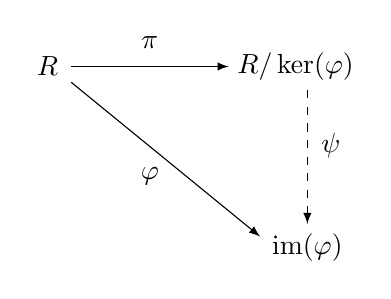
\begin{tikzpicture}
    \draw[-latex] (0, 0) -- (2, 0) node at (-0.3, 0) {$R$} node at (1, 0.3) {$\pi$} node at (2.85, 0) {$R/ \ker(\varphi)$};
    \draw[-latex, dashed] (3, -0.3) -- (3, -2) node at (3, -2.3) {$\im(\varphi)$} node at (3.3, -1) {$\psi$};
    \draw[-latex] (0, -0.2) -- (2.4, -2.16) node at (1, -1.4) {$\varphi$};
  \end{tikzpicture}
\end{center}

Homomorfismen $\pi$ i diagramet ovan är egentligen irrelevant för oss. Poängen med den är att visa att det finns två vägar som leder oss 
till $\im(\varphi)$. Antigen tar man den raka vägen genom $\varphi$ eller så tar man först $\pi$ och sedan $\psi$ och eftersom 
de båda vägarna leder oss till samma slutresultat kan vi konstatera att $\varphi = \psi \circ \pi$ och vi säger att 
diagramet är kommutativt. Satsen ovan bevisar just 
att det faktiskt existerar en $\psi$ som har sådana egenskaper. 

Denna sats är inte unik för ringar och kan tillämpas på grupper också. Nedan följer några roliga exempel på hur man kan visa att 
två grupper är isomorfa med denna sats. 
\begin{exmp}
  Visa att 
  \[\mathbb{R}^*/\{1, -1\} \cong \mathbb{R}^+\]
  där $\mathbb{R}^*$ är gruppen av alla nollskilda reella tal under multiplikation och där $\mathbb{R}^+$ är gruppen av alla positiva reella tal under mutliplikation.

  Definera $\varphi: \mathbb{R}^* \rightarrow \mathbb{R}^+$ genom $\varphi(x) = |x|.$
  Denna är en homomorfism eftersom 
  \[\varphi(x \cdot y) = |x \cdot y| = |x| \cdot |y| = \varphi(x) \cdot \varphi(y).\]
  Observera att $\im(\varphi) = \mathbb{R}^+$ och att $\ker(\varphi) = \{1, -1\}$ eftersom $1$ är enhetselementet i $\mathbb{R}^+$. Vi får då att 
  \[\mathbb{R}^* / \{1, -1\} \cong \im(\varphi) = \mathbb{R}^+.\] 
\end{exmp}

\begin{ovning}{1}
  Låt $\mathbb{R}^2$ vara gruppen av alla reella ordnade par under komponentvis addition $((a, b) + (c, d) = (a + c, b + d))$ och $\mathbb{R}$
  vara gruppen av alla reella tal under addition. Definera 
  \[H = \biggl\{x \cdot (\sqrt 5, -\pi) \; | \; x \in \mathbb{R} \biggr\}.\]
  Visa att $\mathbb{R}^2 / H \cong \mathbb{R}.$
\end{ovning}

Ledning: Åtgå ifrån funktionen $f: \mathbb{R}^2 \rightarrow \mathbb{R}$ som defineras av $f(x, y) = \pi x + \sqrt 5 y$. 
Här finns även en liten genväg som man kan ta genom att skriva upp $f$ i matris form. 

\begin{ovning}{2}
  Visa att en homomorfism $\varphi$ är injektiv om och endast om $\ker(\varphi) = \{0\}.$ Hur kan detta användas för att bevisa att 
  $\psi$ är injektiv i den första isomorfiska satsen?
\end{ovning}

\subsubsection{Kategorisering av ringar}
Detta avnsitt kommer att kategorisera ringar i olika \textit{domäner} som har olika egenskaper. 
Detta är nödvändigt eftersom olika ringar har olika egenskaper. I vissa ringar gäller till exempel att 
$ab = 0$ medför att $a = 0$ eller $b = 0$ medan andra ringar inte har denna egenskap.

\begin{mydef}{Integritetsområden}{}
  En ring $R$ är ett \textit{integritetsområde} om produkten mellan två nollskilda element i $R$ är nollskilt. Det vill säga $ab = 0$ 
  medför att $a = 0$ eller $b = 0$. Vi säger att ett nollskilt och ett icke inverterbart $r \in R$ är \textit{irreducibelt} om 
  faktoriseringen $r = r_1r_2$ kräven att $r_1$ eller $r_2$ är enheter. 
\end{mydef}

\begin{exmp}
  Ringen $\mathbb{Z}_6$ är inte ett integritetsområde eftersom $[2][3] = [6] = 0$. Ringen $\mathbb{Z}$ är därimot ett integritetsområde 
  eftersom $ab = 0$ medför att $a = 0$ eller $b = 0$.
\end{exmp}

\hypertarget{kancelleringslagen}{}
\begin{mytheo}{}{}
  En ring $R$ är ett integritetsområde om och endast om den uppfyller \textit{kancelleringslagen}: om $ra = rb$ för ett nollskilt $r$
  så är $a = b$.
\end{mytheo}

\begin{proof}
  Låt $R$ vara ett integritetsområde och $r, a, b \in R$ för ett nollskilt $r$. Då gäller $r(a -b) = 0$. Eftersom $r \neq 0$
  så måste $a -b = 0$. Detta ger oss att $a = b$. 

  Antag istället att kancelleringslagen gäller för en ring $R$ och låt $r, a$ vara nollskilda element i $R$ så att $ra = 0.$
  Vi noterar att $ra = 0 = r0$ och eftersom kancelleringslagen gäller så är $a = 0$. Detta är dock en motsägelse eftersom $a \neq 0$. 
\end{proof}

\begin{mytheo}{}{}
  $\mathbb{Z}_n$ är ett integritetsområde om och endast om $n$ är ett primtal.
\end{mytheo}
\begin{proof}
  Antag att $\mathbb{Z}_n$ är ett integritetsområde för ett icke primtal $n > 0$. Eftersom $n$ inte är ett primtal så kan vi skriva 
  $n = ab$. Vi vet även att $0 = [n] = [a][b]$ vilket medför att $[a] = 0$ eller $[b] = 0$ eftersom $\mathbb{Z}_n$ är ett integritetsområde. 
  Detta är dock en motsägelse eftersom $1 < a < n$ och $1 < b < n$ och därför kan varken $a$ eller $b$ vara kongruenta med noll mod $n$. 

  Antag istället att $p$ är ett primtal och $[a], [b] \in \mathbb{Z}_p$ så att $0 = [a][b] = [ab]$. Detta medför att 
  $ab \equiv 0 \mod p$ och $p$ måste dela $a$ eller $b$. Detta betyder att $[a] = 0$ eller $[b] = 0$.
\end{proof}

\begin{mydef}{Ringar med entydig faktorisering}{}
  En \textit{ring med entydig faktorisering}, eller EF-ring (eng. \textit{UDF}) är ett integritetsområde där varje element förutom noll och enheter
  kan skrivas entydligt som en produkt av irreducibla element.
\end{mydef}

Denna definition är analog med aritmetikens fundamentalsats, varje heltal större än ett kan skrivas som en unik produkt av primtal. I detta fall sammanfaller 
primtalen med det irreducibla elementen i definitionen ovan och därför är $\mathbb{Z}$ en EF-ring.

\begin{mydef}{Principalidealdomän}{}
  En \textit{principalidealdomän} (PID) är ett integritetsområde där varje ideal genereras av ett element. 
  Det vill säga $I = (a) \equiv \{ar \; | \; r \in R\}$ för ett ideal $I$ till ringen $R$.
\end{mydef}

Vårt mål nu är att visa att varje PID är en EF-ring. För detta behöver vi följande definitioner. 

\begin{mydef}{}{}
  Ett \textit{primelement} $p \neq 0$ är ett element i en ring som inte är en enhet och om $p$ delar $ab$ så måste $p$ dela $a$ eller $b$.
\end{mydef}

Primelement försöker alltså efterlikna vanliga primtal. Notera att primelement och irreducibla element är två olika saker. Ibland kan dock dessa 
sammanfalla med varandra. 
I ringen av heltal $\mathbb{Z}$ är primelementen identiska med primtalen och därför sammanfaller 
de irreducibla element med primelement. 

\begin{mydef}{}{}
  En \textit{Noethersk ring} är en ring $R$ som uppfyller \textit{kedjevillkoret} (eng. \textit{ascending chain condition}, ACC)
  på ideal: givet en kedja av ideal i $R$
  \[ I_1 \subseteq I_2 \subseteq I_3 \subseteq \ldots I_k\]
  så existerar det ett $m$ så att $I_k = I_m$ för $m \leq k$.
\end{mydef}
Med ACC menas alltså att det inte existerar en oändlig lång kedja av ideal där den ena är en \textit{äkta} delmängd av den tidigare. 

Noetherska ringar 
är uppkallade efter den tyska matematikern Emmy Noether som gjorde många viktiga bidrag inom abstrakt algebra. Hon upptänkte bland annat 
Noethers sats som är fundamental inom modern teoretisk fysik och expanderade även konceptet om ideal. 
Noether har även publicerat en artikel om det inversa Galoisproblemet som är ett olösbart problem ännu än idag. Hon har beskrivits av bland annat 
Albert Einstein och Norbert Wiener som den viktigaste kvinnan i matematikens historia. Det finns även många satser som berör Noetherska ringar
såsom Lasker-Noether satsen och Hilberts bassats. Vårt mål är dock att visa att varje PID är EF-ring och vi hoppar därför över detaljerna. 
(Det inversa Galoisproblemet tas dock upp senare.)

\hypertarget{pidnoe}{}
\begin{mytheo}{}{}
  Varje PID är en Noethersk ring. 
\end{mytheo}

\begin{proof}
  Låt $I_1 \subset I_2 \ldots$ vara en kedja av ideal av $R$. Låt $I = \cup_{i = 0}^{\infty} I_i$ och observera att $I$ är ett ideal. Eftersom 
  $R$ är en PID så måste $I = (c)$ för $c \in R$. Eftersom $c \in I$ så måste $c$ även förekomma i ett annat ideal, säg $I_n.$ Då har vi även 
  att $I_n(c)$ och $I_r(c)$ för $r \geq n$. Detta betyder att $I_n = I_m$ som påstått. 
\end{proof}

\hypertarget{inv}{}
\begin{mytheo}{}{}
  Låt $R$ vara en PID. Då är varje nollskilt och icke inverterbart element en produkt av ändligt många irreducibla element.
\end{mytheo}

\begin{proof}
  Låt $a$ vara ett nollskilt och icke inverterbart element i en ring $R$. Vi visar först att $a$ har en irreducibel faktor. 
  Om $a$ är irreducibel så gäller naturligtvist detta. Vi antar därför att $a$ är reducibel, det vill säga $a = a_1b_1$
  där $a_1$ och $b_1$ inte är enheter. Då är $a \in (a_1)$ och $(a) \subset (a_1)$. Denna inneslutning är strikt då 
  om $(a) = (a_1)$ skulle medföra att $a_1b_1n = a_1$ för $n \in R$. Eftersom $R$ är en PID och därför ett integritetsområde
  så gäller \hyperlink{kancelleringslagen}{sats 4.1.2} (kancelleringslagen) 
  som medför att $b_1$ är en enhet, vilket den inte får enligt vårt antagande. 
  Om $a_1$ är reducibelt så kan det skrivas som $a_1 = a_2b_2$ där $a_2$ eller $b_2$ inte är enheter. Med ett liknande argument får vi 
  \[(a) \subset (a_1) \subset (a_2).\]
  Vi kan fortsätta på detta sätt och få en kedja av ideal. Enligt \hyperlink{pidnoe}{sats 4.1.4} så kan dock denna kedja inte vara oändligt lång, 
  det vill säga $I_k = I_m$ för $m \leq k$. Det enda sättet två ideal av vår typ kan vara lika med varandra är om den ena är irreducibel. Detta är 
  lätt att visa och lämnas därför som en övning till läsaren. Detta medför att $(a)$ är en delmängd till $(a_r)$ för ett irreducibelt $a_r \in R$. 
  Detta betyder i sin tur att $a$ måste ha en irreducibel faktor.
  
  Vi visar nu att $a$ är en produkt av ändligt många irreducibla element i $R$. Om $a$ är reducibel kan vi enligt ovanstående 
  skriva $a = p_1c_1$ för ett icke inverterbart element $c_1 \in R$ och ett irreducibelt element $p_1 \in R$. Med argument som 
  liknande dessa i det ovanstående är $(a) \subset (c_1)$. Om $c_1$ är reducibel så kan den skrivas som $c_1 = p_2c_2$ och 
  \[(a) \subset (c_1) \subset (c_2).\]
  Vi kan sedan kolla om $c_2$ är reducibel eller inte osv. Enligt \hyperlink{pidnoe}{sats 4.1.4} kan denna kedja inte vara ändlig och 
  måste sluta med $(c_r)$ för ett irreducibelt $c_r \in R$. Vi har då att $a = p_1p_2 \cdots p_rc_r$ där alla $p_i$ är irreducibla.
\end{proof}

\hypertarget{max}{}
\begin{mylemma}{}{}
  Låt $I$ vara ett ideal till PID'en $R$. Då är $I$ maximal om och endast om $I = (p).$
\end{mylemma}

\begin{proof}
  Antag att $I$ är ett maximalt ideal till PID'en $R$. Då gäller $I = (n)$. Antag att $n$ är reducibel, det vill säga 
  $n = ab$ där $a$ och $b$ inte är enheter. Då gäller $(n) \subset (a)$. Vi observerade i \hyperlink{inv}{sats 4.1.5} att denna inneslutning är strikt.
  Vi vet även att $(a) \neq R$ eftersom $a$ inte är en enhet. Detta är dock en motsägelse eftersom vi antog att $(n)$ var det maximala idealet.

  Antag istället att $p$ är irreducibelt och låt $I_1$ vara det minsta idealet så att $(p) \subset I_1$. Då gäller $I_1 = (q)$ för något $q \in R$. 
  Detta ger oss $p = qn$ för ett $n \in R$. Eftersom $p$ är irreducibelt så måste antigen $q$ vara en enhet eller $n$ vara en enhet. 
  I det första fallet får vi att $I_1 = (q) = R$, vilket är enkelt att visa. I det andra fallet får vi att $q = n^{-1}p$ vilket medför att 
  $q \in (p)$ och $(q) = (p)$, vilket är enkelt att visa. Detta ger oss att $I_1 = I$.
\end{proof}

\hypertarget{maxprim}{}
\begin{mylemma}{}{}
  Det maximala idealet av ringen $R$ är ett primideal.
\end{mylemma}

\begin{proof}
  Låt $M$ vara det maximala idealet av $R$. Antag att $M$ inte är ett primideal. Då existerar det $a, b \in R$ så att produkten 
  $ab$ finns i $M$ men $a \notin M$ och $b \notin M$. Observera att $(a) + M = \{ra + m \; | \; r \in R, \; 0m \in M\}$ är ett ideal av $R$. 
  Eftersom $M \subset (a) + M$ så måste $(a) + M = R$ eftersom $M$ är maximal. Eftersom $1 \in R = (a) + M$ så måste det finnas ett 
  $r \in R$ och $m \in M$ så att 
  \[1 = ra + m.\]
  På samma sätt får vi att $R = (b) + M$ och
  \[ 1 =  sb + n\]
  för $s \in R$ och $n \in M$. 
  Vi får då följande ekvation: 
  \[1 = 1 \cdot 1 = (ra + m)(sb + n) = rasb + ran + msb + mn\]
  och eftersom $ab, m, n \in M$ så tillhör ovanstående ekvation $M$. Detta betyder dock att $1 \in M$ vilket i sin tur betyder 
  att $M = R$ enligt resultat som härledes direkt efter definitionen av ringar. Detta är dock en motsägelse eftersom 
  det maximala idealet är per definition inte lika med hela ringen.
\end{proof}

\hypertarget{irprim}{}
\begin{mylemma}{}{}
  De irreducibla elementen sammanfaller med primelementen i en PID.
\end{mylemma}

\begin{proof}
  Låt $a$ och $b$ vara element i en PID $R$ där $a$ eller $b$ är enheter och $p$ ett irreducibelt element i $R$ så att $p = ab$. Enligt 
  \hyperlink{max}{lemma 4.1.1} och \hyperlink{maxprim}{lemma 4.1.2} så är $(p)$ ett primideal och eftersom $p = ab$ så är $ab \in (p)$.
  Detta medför att $a \in (p)$ eller $b \in (p)$ vilket ger att $p$ delar $a$ eller att $p$ delar $b$. Det irreducibla elementet $p$
  är alltså ett primelement och beviset är slutfört.
\end{proof}

\begin{mytheo}{}{}
  Varje PID är en EF-ring.
\end{mytheo} 

\begin{proof}
  Låt $R$ vara en PID. Enligt \hyperlink{inv}{sats 4.1.5} kan varje element skrivas som en produkt av irreducibla element i $R$. Det som 
  återstår att visa är att denna faktorisering är unik. Antag motsatsen. Då gäller för $a \in R$ att 
  \[ a = p_1p_2 \cdots p_r \quad \textnormal{och} \quad a = q_1q_2 \cdots q_s\]
  för alla irreducibla $p_i$ och $q_j.$ Antag även, utan förlust av generalitet, att $s \geq r.$ Då delar $p_1$ produkten $q_1 \cdots q_s.$
  Enligt \hyperlink{irprim}{lemma 4.1.3} är då $p_1$ ett primelement och då måste $p_1$ dela något annat element, säg $q_j.$
  Notera nu att produkten $q_1 \cdots q_s$ är i en slumpmässig ordning och att vi alltid kan ändra ordningen. Till exempel kan vi byta ordningen 
  så att $q_j$ blir först i denna ordning, det vill säga $q_j = q_1$. 
  Då måste $p_1$ dela $q_1$ och då gäller att $q_1 = u_1p_1$ för en enhet $u_1 \in R.$ Vi får då att 
  \[ p_1p_2 \cdots p_r = u_1p_1q_2 \cdots q_s \]
  och eftersom en PID är per definition ett integritetsområde så gäller 
  \[ p_2 \cdots p_r = u_1 q_2 \cdots q_s. \]
  Genom att fortsätta på detta sätt fås
  \[ 1 = u_1u_2 \cdots u_r q_{r+1} \cdots q_s. \]
  Eftersom $1$ är irreducibelt ($1 = 1 \cdot 1$ och $1$ är en enhet) så måste alla $q_i$ vara enheter. Dessa är dock irreducibla och därför måste 
  $r = s.$ Detta betyder att alla $u_i = 1$ som slutför beviset.
\end{proof}

\begin{mytheo}{}{}
  Varje PID är en $gcd$ \textit{domän}, det vill säga två element har en största gemensam nämnare. 
\end{mytheo}

\begin{proof}
  Låt $a$ och $b$ vara element i en PID $R$. Betrakta idealet som genereras av $a$ och $b$: $(a, b) \equiv \{ ac_1 + bc_2 \; | \; c_1, c_2 \in R \}$.
  Det är enkelt att visa att detta är ett ideal. En bra övning är att visa att ett ideal av en PID som genereras av ändligt många element faktiskt 
  är ett ideal. Eftersom $R$ är en PID så måste $(a, b) = (d)$. Notera att både $a$ och $b$ är element i $(a, b) = (d)$. Detta betyder att 
  $d$ delar $a$ och att $d$ delar $b$. Vi visar nu att $d$ är den \textbf{största} elementet som delar både $a$ och $b$. 

  Antag att $c$ delar $a$ och $b$. Då gäller $a = k_1c$ och $b = k_2c$ för $k_1, k_2 \in R$ och eftersom $(a, b) = (d)$ så är $an_1 + bn_1 = d$
  för $n_1, n_2 \in R$. Detta ger att $d = k_1cn_1 + k_2cn_1$ och $c$ delar alltså $d$ och därför är $d$ den största gemensamma nämnaren till $a$ och $b$.
\end{proof}

\hypertarget{Bézouts identitet}{}
\begin{mykol}{Bézouts identitet}{}
  I en $\gcd$ domän $R$ kan den största gemensamma delaren $d$ till två element $a$ och $b$ i $R$ skrivas som $d = an_1 + bn_2$
  för $n_1, n_2 \in R.$
\end{mykol}
\begin{exmp}
  Bézouts identitet gäller för heltalen. Till exempel så är den störtsa gemensamma nämnaren till $12$ och $42$ $6$ och 
  $6 = 12 \cdot 18 + 42 \cdot (-5).$ En bra övning är att bevisa detta mer formellt. 
\end{exmp}

\begin{mydef}{}{}
  \begin{enumerate}[(i)]
    \item En \textit{Euklidisk värdering} på ett integritetsområde $R$ är en funktion 
    \[ \grad: R \setminus 0 \rightarrow \mathbb{N} \]
    så att 
    \begin{enumerate}
      \item för alla $a$ och $b$ i $R$ med $b$ nollskilt finns $k$ och $r$ i $R$ så att $a = bk + r$ där $r$ antigen är noll eller $\grad (r) < \grad (b),$
      \item för alla nollskilda $a$ och $b$ gäller att $\grad (a) \leq \grad (ab).$
    \end{enumerate}
    \item Ett \textit{Euklidiskt område} är ett integritetsområde som kan utrustas med åtminstånde en Euklidisk värdering.
  \end{enumerate}
\end{mydef}

Ett Euklidiskt område generaliserar alltså den Euklidiska divisionen för heltal. I sådana ringar kan vi använda oss av Euklides algoritm för 
att hitta den största gemensamma delaren till två tal. Den Euklidiska värderingen betecknas i denna text med $\grad$. Detta är praktiskt 
då vi så småningom ska gå vidare till polynom. Vissa författare väljer dock att beteckna den med $f$ eller $d$ och $\grad$ är ingen fastställd beteckning.
\begin{exmp}
  Ringen av heltal $\mathbb{Z}$ är ett Euklidiskt område med den Euklidiska värderingen $\grad (n) = |n|.$
\end{exmp}

\begin{myprop}{}{}
  Ett Euklidiskt område är också en PID.
\end{myprop}
\begin{proof}
  Låt $R$ vara ett Euklidiskt område med ett ideal $I$. Om $I = \{0\}$ så är $I = (0)$ och propositionen gäller för detta fall. 
  Om $I \neq \{0\}$ så finns det ett nollskilt $a$ i $I$ som har den minsta Euklidiska värderingen. För $b \in I$ gäller då 
  $b = qa + r$ där $r$ antigen är noll eller $\grad (r)  < \grad (a).$ Notera dock att $r = q-ba \in I$ och eftersom $\grad (a)$ är minimal 
  så måste $r = 0$. Detta medför att $b = qa$ och vi får att $I = (a).$
\end{proof}
Vi kan nu göra följande kedja

\scalebox{0.9}{ $\textnormal{Ringar} \supset \textnormal{integritetsområden} \supset \textnormal{gcd domäner} \supset \textnormal{EF-ringar} 
\supset \textnormal{PID} \supset \textnormal{Euklidiska områden}$}

\subsection{Kroppar}
För att börja med Galoisteori så måste vi först ha en plats där vi kan utföra vanlig aritmetik, en \textit{kropp}. Galoisteori kan ses som en studie 
av dessa platser som tillåter grundläggande aritmetik och dess relation till polynom. Vi skall i detta delavsnitt och i avsnittet "kroppsutvidgningar" 
presentera de huvudsakliga faktan om 
sådana strukturer. 

\begin{mydef}{Kroppar}{}
    En \textit{kropp} är en mängd $F$ under två binära operationer, addition ($+$) och multiplikation ($\cdot$), som uppfyller följande \textit{kroppsaxiom}.
    \begin{enumerate}[I)]
        \item \textbf{Assosiativitet.} $a + (b + c) = (a + b) + c$ och $a \cdot (b \cdot c) = (a \cdot b) \cdot c$.
        \item \textbf{Kommutativitet.} $a + b = b + a$ och $a \cdot b = b \cdot a$.
        \item \textbf{Additativa och multiplikativa enhetselementet.} Det existerar två olika element $0$ och $1$ så att $a + 0 = a$ och $a \cdot 1 = a.$
        \item \textbf{Additativ invers.} För alla $a$ så existerar det en \textit{additativ invers} till $a$, som betecknas
        $-a$, så att $a + (-a) = 0$.
        \item \textbf{Multiplikativ invers.} För alla $a \neq 0$ så existerar det en \textit{multiplikativ invers} till $a$, som betecknas $a^{-1}$ eller $1/a$, så att 
        $a \cdot a^{-1} = 1.$
        \item \textbf{Distributivitet av multiplikation över addition.} $a \cdot (b + c) = (a \cdot b) + (a \cdot c)$,
    \end{enumerate}
    för $a, b, c \in F$
\end{mydef}
En kropp skapar alltså en abelsk grupp under addition och kroppen utom $0$ skapar en abelsk grupp under multiplikation. Alternativt kan en kropp sägas
vara en \textbf{kommutativ ring med inverser} (just denna definition kommer att användas i framtiden). 
Om $K$ är en kroppsutvidgning till $F$ så kommer vi säga att $F$ är baskroppen. 

\begin{myprop}{}{}
  Varje kropp är ett integritetsområde.
\end{myprop}

\begin{proof}
  Låt $a$ och $b$ vara element i en kropp $F$ så att $ab = 0$. Antag att, utan förlust av generalitet, att $a \neq 0.$ 
  Då är $b = a^{-1}(ab) = 0$. 
\end{proof}

\begin{mydef}{Karakteristik}{}
  Låt $F$ vara en kropp. Om det existerar ett minsta positiva tal $n$ så att $\underbrace{1 + \cdots + 1}_{n} = 0$ så kallas $n$ för kroppens \textit{karakteristik}.
  Om $n$ inte existerar är karakteristiken för kroppen $0.$
\end{mydef}
Man kan göra en koppling mellan karakteristik och cykliska grupper där alla element genereras genom ett enda element. Om en kropps karakteristik inte är noll
så kan den anses vara "cyklisk". 

\begin{mytheo}{}{}
  Om $p$ är ett primtal så är $\mathbb{Z}_p \cong \mathbb{Z}/p\mathbb{Z}$ en kropp.
\end{mytheo}

\begin{proof}
  Det som skall visas är att $\mathbb{Z}_p$ har inverser. Låt $[a] \equiv a + p \mathbb{Z} \in \mathbb{Z}_p$. Eftersom $p$ är ett primtal och 
  $a < p$ så måste de vara relativt prima. Då gäller 
  \[ 1 = xa + yp  \iff xa = 1 - yp\]
  för $x, y \in \mathbb{Z}_n$. Detta ger då att $xa \equiv 1 \mod p$, det vill säga $[x][a] = 1$. Inversen till 
  $[x]$ är alltså $[a]$ och beviset är slutfört. 
\end{proof}

%ta upp mer om prime subfields och olika domäner.

\subsection{Polynom}
\begin{mydef}{Polynom}{}
  Låt $F$ vara en kropp. Ett \textit{polynom} över $F$ är en ekvation på följande form
  \[f(X) = a_0 + a_1X + a_2X^2 + \cdots a_nX^n\]
  där $n \in \mathbb{N}$ och där \textit{koefficienterna} $a_1, a_2, \ldots, a_n \in F$. 
  Mängden $F[X]$ består av alla polynom vars koeffcienter tillhör $F$. \textit{Graden} för ett polynom är den högsta multipliciteten av den obestämda variablen som 
  förekommer i polynomet och betecknas $\grad f(X)$. (För polynomet ovan är $\grad f(X) = n$.)
\end{mydef}
Trots att $\mathbb{Z}$ inte är en kropp så kommer vi fortfarande beteckna $\mathbb{Z}[X]$ som mängden av polynom med heltals koeffcienter
för att slippa skriva mycket. Notera att $F[X]$ bildar en ring eftersom $F$ är en kropp.

\hypertarget{pid}{}
\begin{myprop}{}{}
  Om $F$ är en kropp så är $F[X]$ ett \textit{principalidealdomän} (PID), dvs. varje ideal $I$ till $F[X]$ är på formen 
  $I = (f(X)) \equiv \{f(X)g(X) \; | \; g(X) \in F[X]\}$ för $f(X) \in F[X].$
\end{myprop}
\begin{proof}
  Låt $I$ vara ett ideal till $F[X]$. Om $I = \{0\}$ så är $I = (0)$ och propositionen gäller för detta fall. Låt $I \neq \{0\}$.
  Då måste det finnas ett polynom i $I$ så att graden för denna är minimal bland alla icke konstanta polynom. Vi kallar detta polynom 
  för $f(X).$ Uppenbarligen är $(f(X)) \subseteq I$ eftersom $I$ är sluten under multiplikation. Låt $g(X) \in I$. 
  Genom att dela $f(X)$ med $g(X)$ fås en kvot och rest: 
  \[g(X) = q(X)f(X) + r(X) \iff r(X) = g(X) - q(X)f(X).\]
  Notera att $r(X) \in I$ och eftersom $\grad f(X)$ är minimal i $I$ så måste $r(X) = 0.$ Detta betyder att $I \subseteq (f(X))$, vilket 
  slutför beviset.
\end{proof}

\begin{mydef}{Irreducibla polynom}{}
  Låt $f(X)$ vara ett polynom över kroppen $F$. Vi säger att $f(X)$ är \textit{irreducibelt} över $F$ om det inte kan faktoriseras som $f(X) = g(X)h(X)$
  för $g(X), h(X) \in F[X]$ vars grad är mindre än $f(X)$. Om faktoriseringen går att åstadkomma säger vi att $f(X)$ är \textit{reducibelt} över $F.$
\end{mydef}
Notera att denna faktorisering beror starkt på vilken kropp en jobbar med. I till exempel $\mathbb{Q}[X]$ finns det endast några "få" polynom som är reducibla
över $\mathbb{Q}[X]$, medan alla polynom över $\mathbb{C}[X]$ är reducibla över $\mathbb{C}[X]$. Det sistnämnda är algebrans fundemental sats och 
bevisas senare i texten.

Nedan följer några exempel på metoder för att visa att polynom är irreducibla. 
(några övningar eller exempel, beroende på vad jag väljer)

\begin{mylemma}{Gauss's lemma}{}
Låt $f(X)$ vara ett polynom med heltals koeffcienter. Då är $f(X)$ irreducibel över $\mathbb{Z}$ om och endast om den är irreducibel över $\mathbb{Q}$.
\end{mylemma}
\begin{proof}
  Det som skall bevisas är följande
  \begin{align*}
    f(X) \textnormal{ är irreducibel över } \mathbb{Z} &\Rightarrow f(X) \textnormal{ är irreducibel över } \mathbb{Q}, \\
    f(X) \textnormal{ är irreducibel över } \mathbb{Q} &\Rightarrow f(X) \textnormal{ är irreducibel över } \mathbb{Z}.
  \end{align*}
  Påståendet är ekvivalent med det kontrapositiva påståendet.
  \begin{align}
    f(X) \textnormal{ är reducibel över } \mathbb{Q} &\Rightarrow f(X) \textnormal{ är reducibel över } \mathbb{Z}, \\
    f(X) \textnormal{ är reducibel över } \mathbb{Z} &\Rightarrow f(X) \textnormal{ är reducibel över } \mathbb{Q}.
  \end{align}
  Påstående (2) är trivial, då $\mathbb{Z}[X]$ är en delmängd till $\mathbb{Q}[X]$ (ett heltal är även ett rationellt tal). Vi bevisar påstående (2),
  att om $f(X)$ är reducibel över $\mathbb{Q}$ så medför detta att den också är reducibel över $\mathbb{Z}$. Anta att
  \begin{equation}
    f(X) = g_1(X)g_2(X)
  \end{equation}
  där $g_1(X), \; g_2(X) \in \mathbb{Q}[X]$. Eftersom koefficienterna för $g_1(X)$ och $g_2(X)$ är rationella tal så kan vi multiplicera med ett
  heltal $n$ i båda led i (3) som delar alla koefficienternas nämnare hos $g_1(X)$ och $g_2(X)$. Vi får då ekvationen
  \begin{equation}
    nf(X) = h_1(X)h_2(X)
  \end{equation}
  där $h_1(X), \; h_2(X) \in \mathbb{Z}[X]$. Bland alla dessa uttryck, välj $n$ till det minsta positiva heltalet
  så att faktoriseringen går att utföra. Vi påstår att $n = 1$ som då kommer att slutföra beviset. Vi antar motsatsen, att $n$ inte är 1. Eftersom 
  $n$ delar alla nämnare hos $g_1(X)$ och $g_2(X)$ så kan det inte vara ett primtal och därför måste ett primtal dela $n$. Kalla detta primtal för $p$, då 
  måste även $p$ dela högerledet, $h_1(X)h_2(X)$, eftersom $p$ delar vänsterledet. Anta att 
  \[h_1(X) = a_0 + a_1X + \cdots + a_lX^l, \quad h_2(X) = b_0 + b_1X + \cdots + b_mX^m.\]
  Vi påstår att $p$ antigen delar alla $a_i$ eller alla $b_i$. Antag motsatsen. Det finns nu två olika motsatser som kan antas.
  \begin{enumerate}[I)]
    \item Antigen delar $p$ några $a_i$ \textit{eller} några $b_i$,
    \item $p$ delar några $a_i$ \textit{och} några $b_i$.
  \end{enumerate}
  Påstående I) är falsk då alla koeffcienter i $h_1(X)h_2(X)$ måste vara delbara med $p$ och om endast några koeffcienter i det ena polynomet 
  är delbara med $p$ men inte i den andra så uppfylls detta inte. 

  Vi antar att påstående II) gäller. Det är då lämpligt att anta att $p$ delar $a_0, a_{1}, \ldots, a_{j-1}$ men inte $a_j$ och att 
  $p$ delar $b_0, b_{1}, \ldots, b_{k-1}$ men inte $b_k$. Observera att
  \[c_{j+k} = a_0b_{j+k} + \cdots + a_{j-1}b_{k+1} + a_jb_k + a_{j+1}b_{k-1} + \cdots + a_{j+k}b_0\]
  är en koeffcient i $f(X)$ och $p$ måste därför dela $c_{j+k}$. Vi vet även att $p$ delar $a_0, a_{1}, \ldots, a_{j-1}, b_0, b_{1}, \ldots, b_{k-1}$ 
  och därför måste $p$ dela $a_j b_k$. Detta leder till en motsägelse eftersom $p$ måste isåfall dela $a_j$ och/eller $b_k$ och vi drar slutsatsen att 
  $p$ delar alla koeffcienter i $h_1(X)$ eller alla koeffcienter i $h_2(X)$. Låt oss anta det förra. Definera nu 
  \[h_1'(X) = \frac{1}{p} h_1(X)\]
  som, enligt det ovanstående antagandet, tillhör $\mathbb{Z}[X].$ Vi kan därför dela (4) med $p$ för att få
  \[\frac{n}{p} f(X) = h_1'(X) h_2(X).\]
  Detta strider mot antagandet att $n$ är minimal och vi kan konstatera att $n=1$. Detta slutför beviset för lemmat.
\end{proof}
\textbf{Kommentar: }I ovanstående bevis delade vi upp "om och endast om" ($\iff$) påståendet i två delar, 
$\Rightarrow$ och $\Leftarrow$ och bevisade dem separat. Eftersom detta tar relativt mycket plats så kommer vi i kommande bevis relaterade till "om och endast om"
skriva $\Rightarrow:$ och $\Leftarrow:$ istället för att skriva upp fallen separat. 
\begin{mytheo}{Eisensteins kriterium}{}
  Låt
  \[f(X) = a_0 + a_1X + \cdots + a_nX^n\]
  vara ett polynom över $\mathbb{Z}$. Om det existerar ett primtal $p$ så att 
  \begin{enumerate}[I)]
    \item $p$ inte delar $a_n$,
    \item $p$ delar $a_0, a_1, \ldots, a_{n-1}$,
    \item $p^2$ inte delar $a_0$,
  \end{enumerate}
  så är $f(X)$ irreducibel över $\mathbb{Q}$.
\end{mytheo}
\begin{proof}
  Enligt Gauss's lemma räcker det med att visa att $f(X)$ är irreducibel över $\mathbb{Z}$. Anta att $f(X) = g_1(X) g_2(X)$ där 
  \[g_1(X) = b_0 + b_1X + \cdots b_kX^k, \quad g_2(X) = c_0 + c_1X + \cdots c_lX^l\]
  för $b_0, b_1, \ldots b_k, c_0, c_1, \ldots, c_l \in \mathbb{Z}.$
  Notera att $a_0 = b_0 c_0$ och därför, enligt II) och III), så måste $p$ dela $b_0$ eller $c_0$ men inte både och. Låt oss anta, utan förlust av 
  generalitet, att $p$ delar $b_0$ men inte $c_0$. Enligt I) så kan $p$ inte dela alla koeffcienter i $g_1(X)$. Detta betyder att det måste existera ett $b_i$ så att $p$ delar
  $b_0, b_1, \ldots, b_{i-1}$ men inte $b_i$ för $i \leq k < n$. Enligt II) har vi då att 
  \[a_i = b_0c_i + b_1c_{i-1} + \cdots + b_{i-1}c_1 + b_ic_0\]
  är delbart med $p$. Detta medför att $p$ delar $b_i c_0$, vilket är omöjligt enligt tidigare antaganden.
  Denna motsägelse slutför beviset.
\end{proof}
(några bra övningar)

\section{Kroppsutvidgningar}
\begin{mydef}{Kroppsutvidgningar}{}
  Låt $F$ och $K$ vara kroppar. Om $F$ är en delmängd till $K$ så är $K$ en \textit{kroppsutvidgning} till $F$ och vi skriver antigen $F \subset K$ eller $K/F$.
\end{mydef}
Denna definition vrider lite på perspektivet. Vanligtvist brukar man börja med en mängd och "jobba sig ner" till något mindre, en delmängd. Här är filosofin bakom detta lite 
annorlunda, man börjar med en mängd för att "jobba sig uppåt" till något större. 

\subsection{Graden för en kroppsutvidgning}
Det första som skall observeras är följande. I dessa punkter är $K$ en kroppsutvidgning till $F$ och $a, b \in F$ samt $x, y \in K$.

\begin{enumerate}[I)]
  \item $K$ skapar en abelsk grupp under addition (det är en kropp),
  \item $a \cdot (b \cdot x) = (a \cdot b) \cdot x$,
  \item $1 \cdot x = x$,
  \item $a \cdot (x + y) = (a \cdot x) + (a \cdot y)$,
  \item $(a + b) \cdot x = (a \cdot x) + (b \cdot x)$.
\end{enumerate}
En kroppsutvidgning kan alltså ses som ett vektorrum över baskroppen. 

\begin{mydef}{Graden för en kroppsutvidgning}{}
  \textit{Graden} för en kroppsutvidgning $K$ till $F$ är kardinaliteten (storleken) av basen för $K$ och betecknas $[K:F]$. Om $[K:F]$ är ändlig så 
  säger vi att $K$ är en \textit{ändlig kroppsutvidgning} till $F$. 
\end{mydef}
Notera att en ändlig kroppsutvidgning inte betyder att kardinaliteten av själva kroppsutvidgningen är ändlig. En ändlig kroppsutvidgning
tyder endast på att kardinaliteten av basen, eller \textit{dimensionen} för vektorrumet som det också kallas, är ändlig. Nedan följer exempel på detta.
(några bra exempel som förtydligar detta.) 

\hypertarget{torn lagen}{}
\begin{mytheo}{Torn lagen (eng. tower law)}{}
  Anta att $F, \; K$ och $L$ bildar ett "torn" av kroppsutvidgningar, $F \subseteq K \subseteq L$. Då gäller
  \[ [L:F] = [L:K] \cdot [K:F]. \]
\end{mytheo}
\begin{proof}
  Vi antar att $[L:K]$ och $[K:F]$ är ändliga. Låt $\{v_1, \ldots, v_m\}$ vara basen för $L$ över $K$ och $\{w_1, \ldots, w_n\}$ vara basen för $K$ över $F$.
  Vi påstår att $B = \{v_iw_j \; | \; 1 \leq i \leq m, \; 1 \leq j \leq n\}$ är basen för $L$ över $F$ som då slutför beviset.

  Eftersom $\{v_1, \ldots, v_m\}$ är basen för $L$ över $K$ så spänner den upp $K$ och därför gäller, för $x \in L$ och $a_1, \ldots, a_m \in K$, att 
  \begin{equation}
    x = \sum_{i = 1}^m a_i v_i.
  \end{equation}
  Vi använder nu faktumet att $\{w_1, \ldots, w_n\}$ spänner upp $K$ över $F$ för att få, för 
  \linebreak
  $b_{1i}, \ldots, b_{ni} \in F$,
  \begin{equation}
    a_i = \sum_{j = 1}^n b_{ji}w_j.
  \end{equation}
  Ekvation (6) i (5) mynnar ut i att
  \[x = \sum_{i = 1}^m \sum_{j = 1}^n b_{ji}w_jv_i\]
  och vi drar slutsatsen att $B$ spänner upp $L$ över $F$. Anta nu det existerar ett $c_{ji} \in F$ så att 
  \[\sum_{i = 1}^m \sum_{j = 1}^n c_{ji}w_jv_i = 0.\]
  Vi skriver om detta som 
  \[\sum_{i = 1}^m \biggl( \sum_{j = 1}^n c_{ji}w_j \biggl) v_i = 0\]
  och använder informationen att $c_{ji}w_j \in K$ och att $\{v_1, \ldots, v_m\}$ är basen för $L$ över $K$ för att härleda
  \[\sum_{j = 1}^n c_{ji}w_j = 0.\]
  Eftersom $\{w_1, \ldots, w_n\}$ är basen för $K$ över $F$ så gäller det att $c_{ji} = 0$ för alla $j$ och $i$. Vi drar slutsatsen att 
  $B$ verkligen är basen för $L$ över $F$ och beviset är således slutfört. 
\end{proof}

\subsection{Algebraiska kroppsutvidgningar}
\begin{mydef}{Algebraiska kroppsutvidgningar och element}{}
  Låt $K$ vara en kroppsutvidgning till $F$. Ett element $\alpha \in K$ är \textit{algebraisk} över $F$ om det existerar ett polynom $f(X) \in F[X]$ 
  så att $f(\alpha) = 0.$ Vi säger då att $\alpha$ är en lösning till $f(X)$ eller att $\alpha$ är en rot till $f(X).$ Om $\alpha$ inte är algebraisk så säger 
  vi att den är \textit{transcendental.}
  Om varje element i $K$ är algebraiskt så säger vi att $K$ är en \textit{algebraisk kroppsutvidgning} till $F$.
\end{mydef}
Varje element $\alpha$ i en kropp är självklart algebraisk över denna kropp då $\alpha$ är en rot till $X - \alpha \in F[X]$. Uppkommande lemma visar att 
viktigare ett intressantare resultat. 

\hypertarget{algebraiskkropp}{}
\begin{mylemma}{}{}
  Varje ändlig kroppsutvidgning är algebraisk.
\end{mylemma}

\begin{proof}
  Låt $K$ vara en kroppsutvidgning till $F$ med graden $n$ och $\alpha \in K$. Observera att mängden
  \[A = \{1, \alpha, \alpha^2, \ldots, \alpha^n\} \]
  är en delmängd till $K$ och har kardinaliteten $n+1$. Den högsta möjliga mängden innehållande linjärt \textit{oberoende} element från $K$ kan dock endast vara $n$. 
  Detta betyder att $A$ är linjärt \textit{beroende} över $F$. Med detta kan vi konstatera att ekvationen
  \[b_0 + \alpha^1 b_1 + \alpha^2 b_2 + \cdots + \alpha^n b_n = 0\]
  gäller för $b_i \in F$ där några är skiljda från noll. Vi har alltså att $\alpha$ är en lösning till polynomet 
  \[f(X) = b_0 + X^1 b_1 + X^2 b_2 + \cdots + X^n b_n\]
  vilket slutför beviset.
\end{proof}

\subsection{Enkla kroppsutvidgningar och minimala polynom}
\begin{mydef}{}{}
  Låt $K$ vara en kroppsutvidgning till $F$ och $\alpha_1, \ldots, \alpha_n \in K$. Vi skriver  
  \[F(\alpha_1, \ldots, \alpha_n)\]
  för den minsta delkroppen till $K$ som innehåller $F$ och elementen $\alpha_1, \ldots, \alpha_n$. Vi säger att $K$ är en \textit{enkel kroppsutvidgning} till $F$
  om $K = F(\beta), \; \beta \in K.$ Vi säger då att $K$ har erhållits genom att ha \textit{adjungerat} $\beta$ till $F$.
\end{mydef}
Med denna definition kan vi nu alltid skapa kroppsutvidgningar genom att bara lägga till element i en kropp. 

\begin{mydef}{Minimala polynom}{}
  Låt $K$ vara en kroppsutvidgning till $F$ och $\alpha$ vara ett element i $K$ som är algebraiskt över $F$. Det \textit{minimala polynomet} av $\alpha$ över $F$
  är det moniska polynomet (ett nollskilt polynom med en högstagradskoefficient som är 1) $f(X)$ med lägsta grad i $F[X]$ så att $\alpha$ är en lösning till den. 
\end{mydef}
(exempel)

Nedan följer några viktiga egenskaper hos minimala polynom.
\hypertarget{minpol}{}
\begin{mytheo}{}{}
  Låt $F$ vara en kropp och $\alpha$ ett element i en kroppsutvidgning till $F$ så att $\alpha$ är algebraisk över $F$. Då gäller följande 
  \begin{enumerate}[(i)]
    \item Funktionen $\varphi: F[X] \rightarrow F(\alpha)$ som ges av $\varphi: g(X) \mapsto g(\alpha)$ är en homomorfism med $\ker(\varphi) = (f(X)),$
    \item minimala polynomet $f(X)$ av $\alpha$ över $F$ existerar,
    \item det minimala polynomet $f(X)$ av $\alpha$ över $F$ är irreducibel över $F$.
    \item om $g(X) \in F[X]$ så är $g(\alpha) = 0$ om och endast om minimala polynomet $f(X)$ av $\alpha$ över $F$ delar $g(X),$
    \item det minimala polynomet $f(X)$ till $\alpha$ över $F$ är unik, 
    \item om $g(X) \in F[X]$ är ett moniskt polynom så att $g(\alpha) = 0$ så är $g(X)$ minimala polynomet till $\alpha$ över $F$ om och endast 
    om $g(X)$ är irreducibel över $F$.
  \end{enumerate}
\end{mytheo}

\begin{proof}
  (i) Notera att 
  \[\varphi(g_1(X) + g_2(X)) = g_1(\alpha) + g_2(\alpha) = \varphi(g_1(X)) + \varphi(g_2(X))\]
  och att 
  \[\varphi(g_1(X) g_2(X)) = g_1(\alpha) g_2(\alpha) = \varphi(g_1(X)) \varphi(g_2(X)).\]
  Detta visar att $\varphi$ är en homomorfism. Enligt \hyperlink{isomorfiska}{den första isomorfiska satsen} vet vi då att $\ker(\varphi)$ är ett ideal 
  till $F[X]$. Vidare vet vi även att $F[X]$ är en PID enligt \hyperlink{pid}{proposition 4.3.1}, vilket gör att 
  \[\ker(\varphi) = (f(X)).\]
  Detta leder oss rakt in på (ii).

  (ii) Eftersom $\alpha$ är algebraisk över $F$ så är $\ker(\varphi) \neq \emptyset$. Från (i) har vi att $\ker(\varphi) = (f(X))$
  och i beviset av \hyperlink{pid}{proposition 4.3.1} vet vi även att $f(X)$ har den lägsta graden i $\ker(\varphi)$ bland alla icke konstanta polynom. 
  Eftersom alla element i $F$ har en invers så kan vi dela $f(X)$ med högstagradskoefficienten utan att förändra $(f(X))$. Vi vet även att 
  $f(X) \in \ker(\varphi)$, det vill säga $\varphi(f(X)) = f(\alpha) = 0$. Detta betyder att $f(X)$ är det minimala polynomet av $\alpha$.

  (iii) Antag motsatsen. Då gäller $f(X) = h(X)g(X)$ där graden för $h(X)$ och $g(X)$ är mindre än graden för $f(X)$. Då gäller 
  \[0 = f(\alpha) = g(\alpha) h(\alpha)\]
  och eftersom $F$ är en kropp (mer specifikt är varje kropp ett \textit{integritetsområde}, för $a$ och $b$ tillhörande detta område och 
  $ab = 0$ så måste $a = 0$ eller $b = 0$. Försök att bevisa att varje kropp är ett integritetsområde!) så måste antigen 
  $g(\alpha) = 0$ eller $h(\alpha) = 0$. Detta strider dock mot antagandet att $f(X)$ har den lägsta graden med $\alpha$ som lösning. 

  (iv) Detta följer direkt från (ii): $g(\alpha) = 0 \iff g(X) \in \ker(\varphi) = (f(X))$ detta gäller om och endast om $f(X) \; | \; g(X).$ 
  
  (v) Antag motsatsen. Då existerar det ett moniskt polynom $g(X) \in F[X]$ så att $g(\alpha) = 0$ som har samma grad som $f(X)$. 
  Eftersom $g(X) \in \ker(\varphi)$ så måste 
  \[g(X) = q(X) f(X)\]
  och eftersom $g(X)$ och $f(X)$ har samma grad så måste $q(X)$ vara ett konstant polynom. Vidare vet vi även att $g(X)$ och $f(X)$ är moniska 
  och därför är $q(X) = 1$, det vill säga $g(X) = f(X)$.

  (vi) $\Rightarrow:$ Det minimala polynomet av $\alpha$ över $F$ är irreducibel över $F$ enligt (iii). 
  $\Leftarrow:$ Enligt (iv) kan $g(X)$ skrivas som 
  \[g(X) = q(X)f(X)\]
  och eftersom $g(X)$ är irreducibel och $f(X)$ inte konstant så måste $q(X)$ vara konstant. Faktumet att $g(X)$ är monisk leder till att 
  $q(X) = 1$ och vi har att $g(X) = f(X).$
\end{proof}

\begin{mylemma}{Bézouts identitet för polynom}{}
  Låt $F$ vara en kropp och $f(X), \; g(X) \in F[X]$. Den största gemensamma delaren till $f(X)$ och $g(X)$, dvs. gcd$(f(X), g(X)) = d(X)$, kan skrivas som 
  \[d(X) = a(X)f(X) + b(X)g(X).\]
\end{mylemma}

\begin{proof}
  Notera först att 
  \[A = \{ a(X)f(X) + b(X)g(X) \; | \; a(X), b(X) \in F[X] \}\]
  är ett ideal till $F[X]$ och $A$ kan således skrivas som $A = (d(X)),$ ty $F[X]$ är en PID. Detta betyder i sin tur att 
  $d(X) = a(X)f(X) + b(X)g(X)$. Vi visar nu att $d(X)$ faktiskt är den största gemensamma delaren till $f(X)$ och $g(X)$.
  
  Om $c(X)$ delar både $f(X)$ och $g(X)$ så gäller $f(X) = n(X)c(X)$ och $g(X) = m(X)c(X)$ vilket betyder att 
  $d(X) = a(X)n(X)c(X) + b(X)m(X)c(X)$ och $c(X)$ delar alltså $d(X)$. Vi konstaterar att $d(X)$ är den största gemensamma delaren som 
  slutför beviset.
\end{proof}

\hypertarget{5.3.2}{}
\begin{mytheo}{}{}
  Låt $F$ vara en kropp och $\alpha$ ett element i en kroppsutvidgning till $F$. Den enkla kroppsutvidgningen $F(\alpha)$ till $F$ är en 
  ändlig kroppsutvidgning om och endast om $\alpha$ är algebraisk över $F$. Då detta är uppfyllt gäller även, för det minimala polynomet $f(X)$ av $\alpha$, att
  \begin{equation}
    [F(\alpha) : F] = \grad f(X).
  \end{equation}
  Vidare gäller även 
  \begin{equation}
    F[X]/(f(X)) \cong F(\alpha).
  \end{equation}
\end{mytheo}
\begin{proof}
  (7) 
  
  $\Rightarrow:$ Om $F(\alpha)$ är en ändlig kroppsutvidgning så gäller \hyperlink{algebraiskkropp}{lemma 5.2.1} och $F(\alpha)$ är således algebraisk. 
  
  $\Leftarrow:$ Antag att $\alpha$ är algebraisk över $F$. Notera att om $b \in F(\alpha)$ så kan $b$ skrivas som $b = g(\alpha)$ för $g(X) \in F[X].$
  Genom att dela $f(X)$ med $g(X)$ fås en kvot och rest: 
  \[g(X) = q(X)f(X) + r(X).\]
  Då gäller 
  \[b = g(\alpha) = r(\alpha)\]
  eftersom $f(\alpha) = 0$. Vidare vet vi att graden för $r(X)$ kan maximalt vara $n-1$ för $n = \grad f(X)$. Detta betyder att $B = \{1, \alpha, \ldots, \alpha^{n-1}\}$
  spänner upp $F(\alpha)$. Notera även att $B$ måste vara linjärt oberoende eftersom $n-1 < \grad f(X) = n.$ Detta medför att $B$ är basen för $F(\alpha)$ över $F$, 
  det vill säga 
  \[ [F(\alpha): F] = |B| = n = \grad f(X) \]
  och eftersom $\grad f(X)$ är ändlig så är $F(\alpha)$ också en ändlig kroppsutvidgning. 

  (8) Enligt \hyperlink{minpol}{sats 5.3.1} (i) är $\varphi: F[X] \rightarrow F(\alpha)$ definerad av $\varphi: g(X) \mapsto g(\alpha)$ 
  en homomorfism med $\ker(\varphi) = (f(X)).$ Vi visar nu att $\im(\varphi) = \{g(\alpha) \; | \; g(X) \in F[X]\}$ är en kropp, 
  dvs. att det finns multiplikativa inverser i $\im(\varphi)$. 

  Genom att dela $f(X)$ med $g(X) \in F[X]$ fås en kvot och rest: 
  \[g(X) = q(X)f(X) + r(X)\]
  vilket ger att 
  \[g(\alpha) = r(\alpha)\]
  och eftersom $\grad \; r(X) < \grad f(X)$ så måste $g(X)$ och $f(X)$ vara relativt prima. Enligt \hyperlink{Bézouts identitet}{Bézouts identitet}
  får vi därför 
  \[1 = a(X)f(X) + b(X)g(X)\]
  vilket ger att 
  \[1 = b(\alpha)g(\alpha)\]
  och därför är $b(\alpha)$ inversen till $g(\alpha)$ och $\im(\varphi)$ är således en kropp. Det är uppenbart att $\im(\varphi) = F(\alpha)$
  och enligt \hyperlink{isomorfiska}{den första isomorfiska satsen} så gäller 
  \[F[X]/(f(X)) \cong F(\alpha)\]
  vilket slutför beviset.
\end{proof}
Vi minns från \hyperlink{isomorfiska}{den första isomorfiska satsen} att $\psi:R/\ker(\varphi) \rightarrow \im(\varphi)$ som definerades som 
$\psi: \ker(\varphi) + r \mapsto \varphi(r)$ var den som skapade isomorfismen $R/\ker(\varphi) \cong \im(\varphi)$. Det är även 
den som skapar isomorfismen $F[X]/(f(X)) \cong F(\alpha)$. Om vi använder denna får vi att
\[\psi: \ker(\varphi) + g(X) \mapsto \varphi(g(X)) = g(\alpha)\]
för alla $g(X) \in F[X]$. Detta ger oss följande egenskaper: 
\begin{align*}
  \psi: (f(X)) + a &\mapsto a \\
  \psi: (f(X)) + X &\mapsto \alpha
\end{align*}
för alla $a \in F.$

Vi noterar följande som bevisades i satsen ovan: 
\hypertarget{kol5.3.1}{}
\begin{mykol}{}{}
  Låt $\alpha$ vara algebraisk över kroppen $F$ och $f(X)$ vara det minimala polynomet av $\alpha$ med grad $n$. 
  Då är $\{1, \alpha, \ldots, \alpha^{n-1}\}$ en bas till $F(\alpha)$ över $F$. 
\end{mykol}

\hypertarget{sats5.3.3}{}
\begin{mytheo}{}{}
  Låt $K$ vara en kroppsutvidgning till kroppen $F$. Då är $K$ en ändlig kroppsutvidgning till $F$ om och endast om $K = F(\alpha_1, \ldots, \alpha_n)$
  för $\alpha_1, \ldots, \alpha_n \in K$ som är algebraiska över $F$.
\end{mytheo}

\begin{proof}
  $\Rightarrow:$ Antag att $K$ är en ändlig kroppsutvidgning till $F$. Om vi låter
  $B = \{\alpha_1, \ldots \alpha_n\}$ vara basen för $K$ över $F$ så är $K = F(\alpha_1, \ldots, \alpha_n)$. Enligt 
  \hyperlink{algebraiskkropp}{lemma 5.2.1} är alla $\alpha_i$ algebraiska över $F$.

  $\Leftarrow:$ Antag att $K = F(\alpha_1, \ldots, \alpha_n)$ där alla $\alpha_i \in K$ är algebraiska över $F$. Vi visar med hjälp av induktion att 
  $[K:F]$ är ändlig. Om $n = 0$ så är $K = F$ och då är $[K:F] = [K:K] = 1$.

  Vi visar nu att $[K:F]$ är ändlig för $K = F(\alpha_1 \ldots, \alpha_{n+1})$. Induktionsantagandet ger att $L = F(\alpha_1, \ldots, \alpha_n)$ 
  är en ändlig kroppsutvidgning till $F$. Notera att $K = F(\alpha_1 \ldots, \alpha_{n+1}) = L(\alpha_{n+1})$ och att det minimala polynomet till $\alpha_n$
  har koeffcienter i $L$. Det sistnämnda medför att $\alpha_n$ är algebraisk över $L$ och \hyperlink{5.3.2}{sats 5.3.2} säger att $[L(\alpha_n):L]$
  är ändlig. Enligt \hyperlink{torn lagen}{torn lagen} har vi då att 
  \[ [K:F] = [L(\alpha):F] = [L(\alpha_n): L] \cdot [L : F]\]
  som är ändligt då $[L(\alpha_n): L]$ och $[L : F]$ är ändliga. 
\end{proof}

\begin{exmp}
  Bestäm $[\mathbb{Q}(\sqrt{2}): \mathbb{\mathbb{Q}}]$ och basen för $\mathbb{Q}(\sqrt{2})$ över $\mathbb{Q}$.

  Enligt \hyperlink{minpol}{sats 5.3.1} (vi) så är $f(X) = X^2-1$ det minimala polynomet till $\sqrt{2}$ eftersom det är monsikt och irreducibelt över $\mathbb{Q}$. 
  Eftersom graden för $f(X)$ är 2 så är, enligt \hyperlink{5.3.2}{sats 5.3.2}, $[\mathbb{Q}(\sqrt{2}): \mathbb{\mathbb{Q}}] = 2.$ Basen för $\mathbb{Q}(\sqrt{2})$ över $\mathbb{Q}$
  är enligt \hyperlink{kol5.3.1}{korollarium 5.3.1} $B = \{1, \sqrt{2}\}$. Detta betyder att varje element i $\mathbb{Q}(\sqrt{2})$ kan uttryckas 
  på formen $a + b\sqrt{2}$ för $a, b \in \mathbb{Q}.$

\end{exmp}

\begin{exmp}
  Bestäm $[\mathbb{Q}(\sqrt{2}, \sqrt{3}): \mathbb{\mathbb{Q}}]$ och basen för $\mathbb{Q}(\sqrt{2}, \sqrt{3})$ över $\mathbb{Q}$.
  Ha kanske med $[\mathbb{Q}(\sqrt{2} + \sqrt{3}): \mathbb{\mathbb{Q}}]$ eller liknande!!!!!!!!!!!!!!!!!!!!!!!!!!!!!!!!!!
  
  !!!!!!!!!!!!!!!!!!!!!!!!!!!!!!!

  !!!!!!!!!!!!!!!!!!!!!!!!!!!!!!!!!!!!!!!!!!!!!!!!!!!!!!!!!!!!!!!!!!!!!!!!!!!!!!!!!!!!!!!!!!!!!!!!!!!!!!!!!!
\end{exmp}

\begin{ovning}{3}
  Visa att $\mathbb{R}[X]/(X^2+1) \cong \mathbb{C}$ med satserna som togs upp i detta kapitel och med den första isomorfiska satsen. 
  (En dålig övning... Trivial. Hitta något annat) 
\end{ovning}

\section{Splittringskroppar och normala utvidgningar}
\subsection{Splittringskroppar}
\begin{mydef}{}{}
  Låt $f(X)$ vara ett polynom över en kropp $F$. Vi säger att en kropp $K$ är en \textit{splittringskropp} för $f(X)$ över $F$ om följande villkor uppfylls. 
  \begin{enumerate}[(i)]
    \item $f(X)$ \textit{splittar} till linjära faktorer över $K$, det vill säga 
    \[f(X) = c \prod_{i=1}^n (X- \alpha_i) = c(X-\alpha_1)(X-\alpha_2)\cdots (X-\alpha_n),\]
    \item om $F \subseteq L \subseteq K$ och $f(X)$ splittar över $L$ så är $L = K.$
  \end{enumerate}
\end{mydef}

\hypertarget{lemma6.0.1}{}
\begin{mylemma}{}{}
  Låt $f(X)$ vara ett polynom över kroppen $F$ som splittar över kroppen $L$. Då är 
  \[K = F(\alpha_1, \alpha_2, \ldots, \alpha_n)\]
  en splittringskropp till $f(X)$ över $F$ där $\alpha$ är rötterna till $f(X)$.
\end{mylemma}

\begin{proof}
  Det är uppenbart att $f(X)$ splittar över 
  \[K = F(\alpha_1, \alpha_2, \ldots, \alpha_n)\]
  om $f(X)$ splittar över $L$ med rötterna $\alpha_1, \alpha_2, \ldots, \alpha_n$. Det som återstår att visa är att 
  $K$ är den minimala kroppen som $f(X)$ splittar över. 

  Antag att $F \subseteq K' \subseteq K$ så att $f(X)$ splittar över $K'$. Då gäller 
  \[f(X) = c(X- \beta_1)(X - \beta_2)\cdots (X - \beta_2)\]
  för $\beta_i \in K'.$ Men eftersom $K' \subseteq K$ så måste $\alpha_i = \beta_i$ eftersom det endast existerar en faktorisering för polynom 
  (detta gäller eftersom alla polynom ringar är EF-ringar. Mer specifikt är en PID (och Euklidiska domäner) EF-ringar. Vi hoppar dock över detaljerna och tar detta 
  faktum som givet.) Detta medför att $K' = K$ eftersom $K$ är den minsta kroppen med elementen $\alpha_i$.
\end{proof}

\subsection{Isomorfi mellan splittringkroppar}
\begin{mydef}{}{}
  Låt $\varphi: F_1 \rightarrow F_2$ och $\psi: F_1(\alpha) \rightarrow F_2(\beta)$ vara isomorfismer mellan kroppar där $F_1 \subseteq F_1(\alpha)$
  och $F_2 \subseteq F_2(\beta)$. 
  Vi säger att $\psi$ \textit{förlänger} (eng. \textit{extends})
  $\varphi$ om $\psi(a) = \varphi(a)$ för alla $a \in F_1$ och vi skriver $\psi |_{F_1} = \varphi.$
\end{mydef}

\hypertarget{6.0.2}{}
\begin{mylemma}{}{}
  Låt $\varphi: F \rightarrow K$ vara en homomorfism mellan två kroppar och $f(X)$ ett irreducibelt polynom över $F[X]$. Definiera $f^{\varphi}(X)$
  som polynomet över $K$ som erhållits genom att verka med $\varphi$ på koeffcienterna i $f(X)$. Låt $\alpha$ vara ett element i en kroppsutvidgning till $F$
  och $\beta \in K$ ett i en kroppsutvidgning till $K$ och låt dessa vara lösningarna till
  $f(X)$ respektive $f^{\varphi}(X)$. Då existerar det en isomorfism $\psi:F(\alpha) \rightarrow K(\beta)$ 
  som förlänger $\varphi$ och $\psi(\alpha) = \psi(\beta).$
\end{mylemma}

\begin{proof}
  Isomorfismen $\varphi: F \rightarrow K$ gör att $\varphi^*: F[X] \rightarrow K[X]$ definierad som 
  \[\varphi^*: \sum_{i = 0}^n a_iX \mapsto \sum_{i = 0}^m \varphi(a_i)X\]
  blir en isomorfism. Notera att $f^{\varphi} = \varphi^*(f(X)).$ Notera även att $f^{\varphi}(X)$ är irreducibel över $K$ eftersom $f(X)$ är irreducibel över $F$.
  Isomorfismen $\varphi^*$ mappar även $(f(X))$ till $(f^{\varphi}(X))$ vilket ger oss att
  \[\tilde{\varphi}: F[X]/(f(X)) \rightarrow K[X]/(f^{\varphi})\]
  definierad som 
  \[\tilde{\varphi}: (f(X)) + g(X) \mapsto (f^{\varphi}(X)) + \varphi(g(X))\]
  blir en isomorfism. Vi observerar följande egenskaper hos $\tilde{\varphi}$:
  \[\tilde{\varphi}(f(X) + X) = (f^{\varphi}(X)) + X\]
  (eftersom $\varphi(1) = 1$)
  \[\tilde{\varphi}(f(X) + a) = (f^{\varphi}(X)) + \varphi(a)\]
  för $a \in F$. Enligt \hyperlink{5.3.2}{sats 5.3.2} har vi även isomorfismerna 
  \begin{align*}
    \psi_1: F[X]/(f(X)) &\rightarrow F(\alpha) \\
    \psi_2: K[X]/(f^{\varphi}(X)) &\rightarrow K(\beta)
  \end{align*}
  med egenskaperna
  \begin{align*}
    \psi_1((f(X)) + a) &= a           & \psi_1((f(X)) + X) &= \alpha \\
    \psi_2((f^{\varphi}(X)) + b) &= b & \qquad \psi_2((f^{\varphi}(X)) + X) &= \beta
  \end{align*}
  för $a \in F$ och $b \in K.$ Notera att $\psi_2 \circ \tilde{\varphi} \circ \psi_1^{-1}$ är en isomorfism (enligt resultat från del I är 
  kompositionen av två bijektioner också en bijektion. Att operationerna blir bevarade är enkelt att visa och läsaren får fylla i detaljerna)
  från $F(\alpha)$ till $K(\beta)$ som uppfyller 
  \begin{align*}
    (\psi_2 \circ \tilde{\varphi} \circ \psi_1^{-1}) (a) &= (\psi_2 \circ \tilde{\varphi}) ( (f(X)) + a) = \psi_2 ((f^{\varphi}(X)) + \varphi(a)) = \varphi(a), \\
    (\psi_2 \circ \tilde{\varphi} \circ \psi_1^{-1}) (\alpha) &= (\psi_2 \circ \tilde{\varphi}) ((f(X)) + X) = \psi_2((f^{\varphi}(X)) + X) = \beta.
  \end{align*}
  Isomorfismen $\psi_2 \circ \tilde{\varphi} \circ \psi_1^{-1}$ uppfyller alltså våra önskade villkor och beviset är slutfört.
\end{proof}

\hypertarget{sats6.0.1}{}
\begin{mytheo}{}{}
  Låt $\varphi: F_1 \rightarrow F_2$ vara en isomorfism mellan två kroppar och $f(X)$ ett polynom i $F_1[X]$. Beteckna 
  $f^{\varphi}(X)$ för polynomet över $F_2[X]$ som erhållits genom att ha verkat med $\varphi$ på koeffcienterna i $f(X)$. Låt 
  $K_1$ vara en splittringskropp för $f(X)$ och $K_2$ en splittringskropp för $f^{\varphi}(X).$ Då existerar det en isomorfism $\Psi: K_1 \rightarrow K_2$
  som förlänger $\varphi.$
\end{mytheo}

\begin{proof}
  Låt $n = \grad f(X)$. Vi använder induktion för att bevisa satsen. För $n = 1$ så är $K_1 = F_1$ och $K_2 = F_2$. Vi kan då välja 
  $\Psi$ till $\varphi$ och satsen gäller för detta fall. 

  Vi antar att satsen gäller för ett heltal $n$. Det finns nu två fall för $f(X)$, antigen är den irreducibel över $F_1$ eller inte. Vi hanterar dessa fall separat
  med avseende på att visa att satsen gäller för $\grad f(X) = n+1$:

  \textbf{Fall 1:} $f(X)$ är irreducibel över $F_1$. 

  Eftersom $K_1$ är en splittringskropp för $f(X)$ så kan vi hitta en rot $\alpha \in K_1$ till $f(X)$. Detta gör att faktoriseringen 
  \[f(X) = (X-\alpha)g(X)\]
  går att åstadkomma för ett polynom $g(X)$ med koeffcienter från $F_1(\alpha)$ och med graden $n$. Eftersom $K_1$ har erhållits genom att ha adjungerat $\alpha$ 
  och alla rötter till $g(X)$ så är $K_1$ en splittringskropp för $g(X)$ över $F_1(\alpha)$ enligt \hyperlink{lemma6.0.1}{lemma 6.0.1}.
  Enligt \hyperlink{6.0.2}{lemma 6.0.2} så existerar det en isomorfism 
  $\psi: F_1(\alpha) \rightarrow F_2(\beta)$ så att $\psi |_{F_1} = \varphi$ och $\psi(\alpha) = \beta.$ Genom att verka på $\psi$ på koeffcienterna i $f(X)$
  så får vi 
  \[f^{\varphi}(X) = (X - \beta)g^{\psi}(X)\]
  som ger oss att $K_2$ är en splittringskropp för $g^{\psi}(X)$ över $F_1(\beta)$. Enligt induktionsantagandet existerar det då en isomorfism $\Psi: K_1 \rightarrow K_2$
  så att $\Psi |_{F_1(\alpha)} = \psi$ och eftersom $F_1 \subset F_1(\alpha)$ så gäller 
  \[\Psi |_{F_1} = \psi |_{F_1} = \varphi\]
  dvs. $\Psi(a) = \psi(a) = \varphi(a)$ för alla $a \in F_1$

  \textbf{Fall 2:} $f(X)$ är reducibel över $F_1$.

Vi skriver $f(X) = g(X)h(X)$ för $g(X)h(X) \in F_1[X]$ vars grad är mindre än $n = \grad f(X)$. Vi verkar med $\varphi$ på $f(X)$ för att få 
\[f^{\varphi}(X) = g^{\varphi}(X)h^{\varphi}(X). \]
Låt $\alpha, \ldots, \alpha_k$ vara rötter till $g(X)$ och $\beta, \ldots, \beta_k$ vara rötter till $g^{\varphi}(X).$
Enligt \hyperlink{lemma6.0.1}{lemma 6.0.1} så är då $L_1 = F_1(\alpha, \ldots, \alpha_k)$ splittringskroppen för $g(X)$ och 
$L_2 = F_2(\beta, \ldots, \beta_k)$ splittringskroppen för $g^{\varphi}(X).$ Enligt induktionsantagandet existerar det en 
isomorfism $\psi: L_1 \rightarrow L_2$ så att $\psi |_{F_1} = \varphi.$

Vi noterar nu att $K_1$ har erhållits från $F_1$ genom att ha adjungerat alla rötter till $f(X)$. Därför har $K_1$ även erhållits
från $L_1$ genom att ha adjungerat alla rötter till $h(X)$. Detta betyder att $K_1$ är splittringskroppen för $h(X)$ över $L_1$. Ett liknande 
argument visar att $K_2$ är splittringskroppen för $h^{\varphi}(X) = h^{\psi}(X)$ över $L_2$. Enligt induktionsantagandet så existerar det 
en isomorfism $\Psi: K_1 \rightarrow K_2$ så att $\Psi |_{L_1} = \psi$. Eftersom $F_1 \subset L_1$ så gäller 
\[\Psi |_{F_1} = \psi |_{F_1} = \varphi\]
dvs. $\Psi(a) = \psi(a) = \varphi(a)$ för alla $a \in F_1$. 
\end{proof}


\begin{mydef}{}{}
  Låt $F$ vara en kropp och $K_1$ och $K_2$ kroppsutvidgningar till $F$. En \textit{F-isomorfism} från $K_1$ till $K_2$ är en isomorfism 
  $\varphi: K_1 \rightarrow K_2$ så att $\varphi(a) = a$ för alla $a \in F.$ Vi säger då att $K_1$ och $K_2$ är $F$-\textit{isomorfa}.
\end{mydef}
I en $F$-isomorfism mellan två kroppsutvidgningar så blir alltså alla element i baskroppen "oberörda" och mappas till säg själva. Med denna definition 
kan vi notera följande korollarium från ovanstående sats och samtidigt dra slutsatsen att splittringskroppar är unika.

\begin{mykol}{}{}
  Låt $f(X)$ vara ett polynom över kroppen $F$. Två splittringskroppar till $f(X)$ är $F$-isomorfa. 
\end{mykol}
\begin{proof}
  Sätt $F_1 = F_2 = F$ och definiera $\varphi(a) = a$ för alla $a \in F$ i \hyperlink{sats6.0.1}{sats 6.0.1}
\end{proof}

\begin{mydef}{}{}
  En \textit{automorfism} av en kropp $F$ är en isomorfism från $F$ till $F$. Låt $K$ vara en kroppsutvidgning till $F$. En $F$-\textit{automorfism} 
  är en $F$-isomorfism från $K$ till $K.$
\end{mydef}
En automorfism kan alltså ses som en permutation av $F$ och en $F$-automorfism kan ses som en permutation där alla element i $F$ blir "oberörda".
\begin{exmp}
  aölskdfjölkasdjfkölasdjfölkasdjflökasdjfölksadfj
\end{exmp}
\begin{exmp}
  aösldkfjöalskdfjöalksdfjöasldfjk
\end{exmp}

\subsection{Normala utvidgningar}
\begin{mydef}{Normala utvidgningar}{}
  En kroppsutvidgning $K$ av en kropp $F$ sägs vara \textit{normal över} $F$ om alla irreducibla polynom över $F$ som har åtminstånde en rot i $K$ splittar 
  över $K$.
\end{mydef}

\begin{exmp}
  Kroppen $\mathbb{C}$ är normal över $\mathbb{R}$ eftersom alla polynom över $\mathbb{R}$ splittar över $\mathbb{C}$ enligt 
  algebrans fundamentalsats. 
\end{exmp}
Med hjälp av följande sats kan fler exempel tas upp. 

\begin{mytheo}{}{}
  En ändlig kroppsutvidgning $K$ av en kropp $F$ är normal om och endast om $K$ är splittringskroppen för något polynom över $F.$
\end{mytheo}
\begin{proof}
  $\Rightarrow$: Antag att $K$ är en ändlig kroppsutvidgning och att den är normal över $F$. Enligt \hyperlink{sats5.3.3}{sats 5.3.3}
  vet vi att $K = F(\alpha_1, \ldots, \alpha_n)$ för alla $\alpha_i \in K$ som är algebraiska över $F.$ Låt $f_i(X)$ vara det minimala polynomet 
  till $\alpha_i$ över $F$ och 
  \[g(X) = f_1(X) f_2(X) \cdots f_m(X).\] 
  Eftersom $f_i(X)$ är irreducibel och har åtminstånde en rot i $K$ så splittar den över $K$ enligt antagandet att $K$ är normal över $F$. Det följder från detta 
  att $g(X)$ splittar över $K$ och eftersom $K$ har erhållits genom att ha adjungerat rötter till $f_i(X)$ så är $K$ splittringskroppen till $g(X).$

  $\Leftarrow:$ Antag istället att $K$ är splittringskroppen för ett polynom $g(X) \in F[X]$. Låt $f(X)$ vara ett irreducibelt polynom över $F$ och antag 
  att $f(X)$ har en rot $\alpha \in K$. Vi skall visa att $f(X)$ splittar över $K$.
  
  Låt $L$ vara splittringskroppen för $f(X)$ över $F$ och $\beta \in L$ en rot till $f(X)$. Följande diagram visar alla kroppsutvidgningar/delkroppar 
  till kropparna som vi jobbar med. 


  \begin{center}
    \newcommand{\mydistance}{.6cm}
    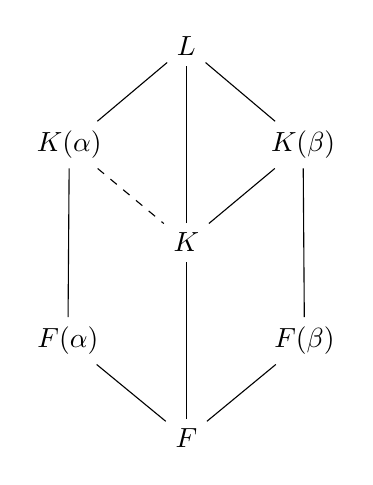
\begin{tikzpicture}[node distance=2cm, scale=1]
    \node(L) {$L$};
    \node(Ka) [below left=1cm of L] {$K(\alpha)$};
    \node(Kb) [below right=1cm of L] {$K(\beta)$};
    \node(K) [below=2cm of L] {$K$};
    \node(F) [below=2cm of K] {$F$};
    \node(Fa) [below left=1 of K] {$F(\alpha)$};
    \node(Fb)[below right = 1 of K] {$F(\beta)$};  

    \draw[dashed](Ka) -- (K);
    \draw(Kb) -- (K);
    \draw(L) -- (Ka);
    \draw(L) -- (Kb);
    \draw(K) -- (L);
    \draw(F) -- (K);
    \draw(Ka) -- (Fa);
    \draw(Fa) -- (F);
    \draw(Fb) -- (F);
    \draw(Kb) -- (Fb);
    \end{tikzpicture}
  \end{center}
  Genom att "jobba oss uppåt" i diagramet hittar vi kroppsutvidgningar och jobbar vi oss ned hittar vi delkroppar. 
  Den streckade linjen ska visa att $K(\alpha) = K$, vilket gäller eftersom $\alpha \in K.$
  Exempelvis är $F(\alpha)$ en kroppsutvidgning 
  till $F$. Vi skall visa att $K(\beta) = K$ som då medför att $\beta \in K$ som slutför beviset. Från diagramet och med \hyperlink{torn lagen}{torn lagen}
  noterar vi följande:
  \begin{align}
    [K(\beta): K] \cdot [K:F] &= [K(\beta): F] = [K(\beta): F(\beta)] \cdot [F(\beta): F] \\
    [K(\alpha): K] \cdot [K:F] &= [K(\alpha): F] = [K(\alpha): F(\alpha)] \cdot [F(\alpha): F].
  \end{align}
  Vidare vet vi även från \hyperlink{5.3.2}{sats 5.3.2} att
  \[[F(\alpha): F] = [F(\beta):F] = \grad f(X)\]
  och att
  \[F(\alpha) \cong F[X]/(f(X)) \cong F(\beta)\]
  eftersom $f(X)$ är irreducibelt och därmed det minimala polynomet till $\alpha$ och $\beta$ enligt \hyperlink{minpol}{sats 5.3.1}. Vi låter 
  $\varphi$ vara funktionen som skapar isomorfismen mellan $F(\alpha)$ och $F(\beta)$. 
  Vi minns att en egenskap hos $\varphi: F[X]/(f(X)) \rightarrow F(\alpha)$ var att det var en $F$-isomorfism.

  Observa nu att $K(\alpha)$ kan erhållas genom att adjungera alla rötter till $g(X)$ till $F(\alpha)$. Detta betyder att 
  $K(\alpha)$ är splittringskroppen för $g(X)$ över $F(\alpha)$ och ett liknande argument visar att $K(\beta)$ är splittringskroppen för 
  $g(X)$ över $F(\beta)$. Enligt \hyperlink{sats6.0.1}{sats 6.0.1} existerar det då en isomorfism $\psi: K(\alpha) \rightarrow K(\beta)$ 
  så att $\psi |_{F(\alpha)} = \varphi$. Observera att $\psi$ mappar $F(\alpha)$ till $F(\beta)$. Detta medför att basen för $K(\alpha)$
  över $F(\alpha)$ blir mappad till basen för $K(\beta)$ över $F(\beta)$ (övertyga dig om detta!). Detta betyder i sin tur att 
  $[K(\alpha):F(\alpha)] = [K(\beta): F(\beta)]$. Detta betyder att vänsterledet i (9) måste vara lika med vänsterledet i (10). Detta ger 
  \[[K(\beta): K] = [K(\alpha):K]\]
  och eftersom $\alpha \in K$ så är $[K(\beta):K] = 1$, vilket betyder att $\beta \in K$ och beviset är slutfört. 
\end{proof}

\section{Separerbarhet}
\subsection{Separerbara polynom}
\begin{mydef}{}{}
  Låt $f(X)$ vara ett irreducibelt polynom över kroppen $F$. Vi säger att $f(X)$ är \textit{separerbart} över $F$ om den inte har flera 
  rötter i dess splittringskropp $K$. Det vill säga 
  \[f(X) = c(X-\alpha_1)c(X-\alpha_1)\cdot (X-\alpha_n)\]
  för \textit{olika} $\alpha_1, \alpha_2, \ldots, \alpha_n \in K.$
\end{mydef}
Det visar sig att det finns en koppling mellan separerbara polynmom och deras första derivata. Därför görs följande definition. 
\begin{mydef}{}{}
  Låt $f(X) = a_0 + a_1X + a_2X^2 + \cdots + a_nX^n$ vara ett polynom över kroppen $F$. \textit{Derivatan} av $f(X)$ är polynomet 
  \[f'(X) = Df(X) = a_1 + 2a_2X + 3a_3X^2 + \cdots na_nX^{n-1}.\]
\end{mydef}
Notera att vi definierar derivatan utan att ens nämna gränsvärden. Av denna anledning har derivatan i detta fall inget att göra med lutningen/tangenten 
till ett polnom. För att kunna utnyttja derivatan måste vi först gå igenom grundläggande egenskaper hos dessa, såsom produktregeln. 

\begin{mylemma}{}{}
  Låt $f(X)$ och $g(X)$ vara polynom över kroppen $F$ och $\alpha, \beta \in F$ skalärer. Då gäller 
  \[ D(\alpha f(X) + \beta g(X))  = \alpha Df(X) + \beta D g(X) \]
  och
  \[ D(f(X)g(X)) = D(f(X))g(X) + D(g(X)) f(X).\]
  Den ovanstående egenskapen benämns \textit{produktregeln.}
\end{mylemma}

\begin{proof}
  Antag att 
  \[f(X) = \sum a_iX^i \quad \textnormal{och} \quad g(X) = \sum b_iX^i.\]
  Då är 
  \[\alpha f(X) + \beta g(X) = \sum (\alpha a_i + \beta b_i)X^i\]
  vilket ger 
  \begin{align*}
    D(\alpha f(X) + \beta g(X)) &= \sum i(a_i + b_i)X^{i-1} \\
    &= \alpha \sum ia_i X^{i-1} + \beta \sum ib_i X^{i-1} \\
    &= \alpha D(f(X)) + \beta D(g(X)).
  \end{align*}
  Innan vi går vidare till produktregeln så kollar vi på ett specialfall. Antag att $f(X) = X^n$ och $g(X) = X^m$. Vi visar nu att 
  produktregeln håller för $f(X)$ och $g(X)$. Notera att 
  \[D(f(X)g(X)) = (n+m)X^{n+m-1}\]
  och att 
  \begin{align*}
    D(f(X))g(X) + D(g(X)) f(X) &= nX^{n-1} \cdot X^m + mX^{m-1} \cdot X^n \\
    &= (n+m)X^{n+m-1}.
  \end{align*}
  Vi använder nu detta specialfall och faktumet att derivatan är linjär för att härleda produktregeln. 
  Låt oss, återigen, anta att
  \[f(X) = \sum a_iX^i \quad \textnormal{och} \quad g(X) = \sum b_iX^i. \]
  Vi observerar följande:
  \begin{align*}
    D(f(X)g(X)) &= D \biggl( \sum_{i, j} a_i b_j X^i X^j\biggr) \\
    &= \sum_{i, j} a_i b_j D(X^iX^j) \quad \textnormal{första delen av lemmat} \\
    &= \sum_{i, j} a_i b_j (D(X^i)X^j + D(X^j)X^i ) \quad \textnormal{specialfallet} \\
    &= \biggl (  \sum a_i D(X^i) \biggr) \biggl (  \sum b_jX^j \biggr) + \biggl ( \sum b_j D(X^j)  \biggr) \biggl ( \sum a_iX^i  \biggr) \\
    &= D \biggl (  \sum a_i X^i \biggr) \biggl (  \sum b_jX^j \biggr) + D \biggl ( \sum b_j X^j  \biggr) \biggl ( \sum a_iX^i  \biggr) \\
    &= D(f(X)) g(X) + D(g(X)) f(X)
  \end{align*}
  som påstått.
\end{proof}

Följande lemma visar kopplingen mellan polynom och dess derivata som kommer att användas vid senare tillfällen. 

\hypertarget{lemma7.2.1}{}
\begin{mylemma}{}{}
  Låt $f(X)$ vara ett polynom över kroppen $F[X]$. Då har $f(X)$ repeterade rötter i dess splittringskropp om och endast om $f(X)$ och $Df(X)$
  har en gemensam faktor som har åtminstånde graden ett i $F[X]$.
\end{mylemma}

\begin{proof}
  $\Rightarrow:$ Antag att $f(X) \in F[X]$ har repeterade rötter i dess splittringskropp $K$. Då gäller 
  \[f(X) = (X-\alpha)^2 g(X)\]
  där $\alpha \in K$ och $g(X) \in K[X].$ Produktregeln ger att 
  \[D(f(X)) = 2(X- \alpha) g(X) + D(g(X)) (X - \alpha)^2\]
  och vi noterar att $f(\alpha) = Df(\alpha) = 0.$ Enligt \hyperlink{minpol}{sats 5.3.1 (iv)} så delar det minimala polynomet till $\alpha$ både 
  $f(X)$ och $Df(X)$. De har alltså en gemensam faktor vars grad är åtminstånde ett. 

  $\Leftarrow:$ Antag att $f(X) \in F[X]$ och $Df(X)$ har en gemensam faktor vars grad är åtminstånde ett. 
  Skriv 
  \[f(X) = \prod_{i = 0}^{\grad f(X)} (X-\alpha_i) \quad \textnormal{och} \quad g(X) = \prod_{j = 0}^{\grad g(X)} (X-\beta_j)\]
  för $\alpha_i$ och $\beta_i$ som tillhör splittringskropparna för $f(X)$ respektive $g(X)$. Eftersom dessa 
  splittringkroppar är kroppsutvidgningar av $F$ så måste $(X - \alpha_a)$ = $(X - \beta_b)$ för några $\alpha_a$ och $\beta_b$ enligt vårt antagande. 
  Vi skriver nu 
  \begin{equation}
    f(X) = (X-\alpha_a)g(X)
  \end{equation}
  för ett polynom $g(X)$ över splittringskroppen för $f(X)$. Enligt produktregeln får vi 
  \[Df(X) = g(X) + (X - \alpha_a)Dg(X).\]
  Vi vet att $(X - \alpha_a)$ måste dela $g(X)$ eftersom $(X - \alpha_a)$ delar $Df(X)$. Detta gör att $g(X)$ kan skrivas som
  \[g(X) = (X - \alpha_a)h(X)\]
  för ett polynom $h(X)$ över splittringskroppen för $f(X)$. Detta i (11) ger 
  \[f(X) = (X - \alpha_a)^2h(X)\]
  och $f(X)$ har således repeterade rötter.
\end{proof}

\begin{myprop}{}{}
  Låt $f(X)$ vara ett irreducibelt polynom över kroppen $F$ som har karakteristik noll. Då är $f(X)$ separerbar. 
\end{myprop}

\begin{proof}
  Antag motsatsen. Enligt \hyperlink{lemma7.2.1}{lemma 7.2.1} så har det irreducibla polynomet $f(X)$ och $Df(X)$ en gemensam faktor. 
  Vi vet dock att graden för $Df(X)$ inte kan vara noll eftersom $f(X)$ inte är konstant och karakteristiken för $F$ är noll. Detta är alltså 
  en motsägelse.
\end{proof}

\begin{mydef}{}{}
  Låt $K$ vara en algebraisk kroppsutvidgning till kroppen $F$. Vi säger att $K$ är en \textit{separerbar utvidgning av} $F$ om 
  det minimala polynomet till varje element i $K$ över $F$ är separerbar över $F$. 
\end{mydef}

\section{Galoisteorins fundamentalsats}
Vi har nu tagt upp förkunskaperna för att börja med Galoisteori. Detta görs dock inte i detta text. Hitta en annan källa lmao f u.
% Det är här den matematiska vackerheten och syftet med hela texten uppträder.
\section{Lösbara grupper och lösningarna till polynom}
\end{document}
